\documentclass[10pt,twoside]{article}

\usepackage[T1]{fontenc}
\usepackage[utf8]{inputenc}
\usepackage{lmodern}
\usepackage{microtype}
\usepackage[a4paper,margin=27mm,headheight=14pt]{geometry}
\usepackage{amsmath,amssymb,amsthm,mathtools}
\usepackage{mathrsfs}
\usepackage{booktabs}
\usepackage{graphicx}
\usepackage{tikz}
\usepackage{pgfplots}
\usepgfplotslibrary{groupplots}
\pgfplotsset{compat=1.17}
\usepackage{enumitem}
\usepackage{xurl}
\usepackage{fancyhdr}
\usepgfplotslibrary{fillbetween}

% Compact table of contents with blue entries and black page numbers.
\usepackage{xcolor}
\usepackage{tocloft}
\renewcommand{\cfttoctitlefont}{\hfill\normalfont\large\scshape}
\renewcommand{\cftaftertoctitle}{\hfill}
\renewcommand{\cftsecfont}{\normalfont\color{blue}}
\renewcommand{\cftsubsecfont}{\normalfont\color{blue}}
\renewcommand{\cftsecpagefont}{\normalfont\color{black}}
\renewcommand{\cftsubsecpagefont}{\normalfont\color{black}}
\renewcommand{\cftsecleader}{\hfill}
\renewcommand{\cftsubsecleader}{\hfill}
\renewcommand{\cftsecaftersnum}{.}
\renewcommand{\cftsubsecaftersnum}{.}
\cftsetindents{section}{0pt}{2em}
\cftsetindents{subsection}{0pt}{2.8em}
\setlength{\cftbeforesecskip}{2pt}
\setlength{\cftbeforesubsecskip}{0pt}
\setlength{\cftbeforetoctitleskip}{0pt}
\setlength{\cftaftertoctitleskip}{8pt}

\usepackage[colorlinks=true,linkcolor=blue,citecolor=blue,urlcolor=blue]{hyperref}

% Running heads in the style of the DLN paper.
% Even pages: abbreviated authors; odd pages: title.
% Page numbers appear at the outer top corners.
\pagestyle{fancy}
\fancyhf{}
\fancyhead[LE,RO]{\small\thepage}
\fancyhead[CE]{\footnotesize P. T. Dang, T. T. Dao, N. M. Doan}
\fancyhead[CO]{\footnotesize The torus with asymptotically the fewest
simple closed geodesics}
\renewcommand{\headrulewidth}{0pt}
\renewcommand{\footrulewidth}{0pt}

% The first page has no running head and a centered page number below.
\fancypagestyle{plain}{%
  \fancyhf{}
  \fancyfoot[C]{\small\thepage}
  \renewcommand{\headrulewidth}{0pt}
  \renewcommand{\footrulewidth}{0pt}
}

\setlength{\parindent}{15pt}
\setlength{\parskip}{1.5pt}
\setlist{nosep}
\allowdisplaybreaks

\theoremstyle{plain}
\newtheorem{theorem}{Theorem}[section]
\newtheorem{proposition}[theorem]{Proposition}
\newtheorem{lemma}[theorem]{Lemma}
\newtheorem{corollary}[theorem]{Corollary}

\theoremstyle{definition}
\newtheorem{conjecture}[theorem]{Conjecture}

\newtheorem{question}[theorem]{Question}

\theoremstyle{remark}
\newtheorem{remark}[theorem]{Remark}

\DeclareMathOperator{\Area}{Area}
\DeclareMathOperator{\arccosh}{arccosh}
\DeclareMathOperator{\arsinh}{arsinh}
\DeclareMathOperator{\Hess}{Hess}
\DeclareMathOperator{\sys}{sys}
\DeclareMathOperator{\tr}{tr}

\newcommand{\A}{\mathcal A}
\newcommand{\B}{\mathcal B}
\newcommand{\R}{\mathbb R}
\newcommand{\Z}{\mathbb Z}
\newcommand{\Xmod}{X_{\mathrm{mod}}}

\title{The torus with asymptotically the fewest
simple closed geodesics}
\author{Phuc Thinh Dang, Trong Toan Dao, Nhat Minh Doan}
\date{}
\begin{document}
\maketitle
\thispagestyle{plain}
% Unnumbered classification footnote on the first page.
\begingroup
\renewcommand{\thefootnote}{}
\begin{NoHyper}
\footnotetext{\textit{2020 Mathematics Subject Classification.}
Primary 30F60; Secondary 53C22, 52A10.\par
\textit{Keywords.} Hyperbolic surfaces, modular torus, simple closed
geodesics, stable norm, McShane--Rivin area conjecture, Farey polygons, Mirzakhani functions.}
\end{NoHyper}
\endgroup

\begin{abstract}
We prove that the modular torus uniquely minimizes the area of the
stable-norm unit ball among complete finite-area hyperbolic
once-punctured tori, resolving the McShane--Rivin area conjecture.
It therefore has fewer simple closed geodesics of length at most $L$
than each fixed nonmodular torus for all sufficiently large $L$.
We also bound the area increase away from the modular torus
and determine the leading growth and first correction term of the
area as the systole tends to zero, uniformly in the twist.
We propose several related questions for further investigation.
\end{abstract}

\setcounter{tocdepth}{1}
\begingroup
\setlength{\parskip}{0pt}
\hypersetup{linkcolor=blue,linktoc=section}
\tableofcontents
\endgroup

\section{Introduction}

Let $S=S_{1,1}$ be a once-punctured torus. Choose an integral homology
basis to identify $H_1(S;\Z)$ with $\Z^2$ and $H_1(S;\R)$ with $\R^2$.
For a complete finite-area hyperbolic structure $X$ on $S$, let
$\|\cdot\|_X$ be its stable norm. For each nonzero primitive class $h\in H_1(S;\Z)$, $\|h\|_X$ is
the length of the unique oriented simple closed geodesic representing
$h$. The classes $h$ and $-h$ represent the same geodesic with
opposite orientations. Set
$$
\B_X=\{w\in\R^2:\|w\|_X\leq1\},
\qquad
\A(X)=\Area(\B_X),
$$
where $\Area$ is the usual Euclidean area. Changes of integral
homology basis have determinant $\pm1$, so $\A(X)$ is independent
of this choice. Isometries preserve the stable norm and the integral
homology lattice, so $\A$ depends only on the isometry class of $X$
and defines a function on the moduli space.

The stable norm belongs to the theory of geometric norms on homology
developed by Federer and Gromov \cite{Federer1974,Gromov1983}.
For a hyperbolic once-punctured torus $X$, McShane and Rivin showed that
its unit-ball area $\A(X)$ determines the leading term in simple-geodesic
counting \cite{McShaneRivinNorm,McShaneRivinTori}. If $N_X(L)$
counts unoriented simple closed geodesics of length at most $L$, then
\begin{equation}\label{eq:Counting}
 N_X(L)=\frac{3}{\pi^2}\A(X)L^2+O_X(L\log L).   
\end{equation}

Thus, minimizing the \emph{McShane--Rivin function} $\A$ asks which hyperbolic torus has the fewest
simple closed geodesics in the asymptotic sense.
For the modular torus $\Xmod$, symmetries and the trace-length
relation connect this counting problem to Zagier's count of Markoff triples
\cite{Zagier1982}, and Risager recently improved the error term in
\eqref{eq:Counting} to $o(L)$ \cite{Risager2026} answering a question of Zagier. For the leading term,
McShane and Rivin conjectured that $\A$ is minimized at $\Xmod$
\cite[Conjecture~3.4]{McShaneRivinTori}.
In his lecture \cite{Bonahon2018}, Bonahon presented
numerical evidence for this conjecture, obtained in joint work
with Enriquez using shear coordinates. 

Mirzakhani extended this counting result to complete finite-area
hyperbolic surfaces of genus $g$ with $n$ cusps and $3g-3+n>0$:
the growth exponent is $6g-6+2n$, and the leading coefficient
is a positive topological constant times the \emph{Mirzakhani function}
\cite{MirzakhaniGrowth}.
This function is the Thurston measure of the compactly supported
measured laminations of length at most one.
With the integral multicurve lattice normalization, on a once-punctured torus, it equals half of the McShane--Rivin function, since each nonzero integral
multicurve corresponds to two opposite homology classes
\cite{MirzakhaniGrowth}.
Continuity and properness ensure that a minimum exists on each
moduli space, but do not identify the minimizing surfaces
\cite[Proposition~3.2 and Theorem~3.3]{MirzakhaniGrowth}.
Arana-Herrera and Athreya refined the estimates near degeneration
and proved square-integrability for Weil--Petersson measure
\cite{AranaHerreraAthreya}. The Weil--Petersson integral of this function is also related to Masur--Veech
volumes through work of Mirzakhani \cite{MirzakhaniEarthquake}
and explicit formulas of Delecroix, Goujard, Zograf, and Zorich
\cite{DelecroixGoujardZografZorich}. 

The function also appears in other counting problems.
For closed surfaces, Rafi and Souto give counting formulas for
mapping class group orbits of filling geodesic currents and for
mapping classes counted using the Thurston metric
\cite{RafiSouto}.
Aougab and Athreya obtain analogous formulas for harmonic
representatives of a fixed weighted triangulation under the
mapping class group, counted by weighted length
\cite[Theorem~1.2]{AougabAthreya}.
For two closed hyperbolic surfaces of the same genus $g\geq2$,
Lowe, Marques, and Neves showed that the leading coefficient
for counting $\pi_1$-injective minimal Lagrangian immersions
of genus $g$ into their product by area is proportional
to the product of their Mirzakhani functions
\cite[Corollary~1.5]{LoweMarquesNeves}. These connections motivate the broader question suggested in
Parlier's survey \cite{ParlierSurvey}: which surfaces minimize
the Mirzakhani function for each topological type? In Subsection~\ref{sec:Further}, we discuss related questions
about other geometric invariants.

\subsection{Main results} In this paper, we prove the McShane--Rivin conjecture, establish uniqueness,
and give quantitative bounds for the increase away from
the modular torus. The symmetry of the modular torus plays an important role in our proof
and may also guide the search for minimizers in higher complexity.

\begin{theorem}
\label{thm:global-area}
Every complete finite-area hyperbolic once-punctured torus $X$ satisfies
$$
\A(\Xmod) \le \A(X),
$$
with equality exactly when $X$ and $\Xmod$ are isometric.
Consequently, if $X$ is not isometric to $\Xmod$, then by \eqref{eq:Counting} $$N_{\Xmod}(L)<N_X(L)$$ for all sufficiently large $L$,
with the threshold depending on $X$.
\end{theorem}

The minimum of $\A$ has consequences for several counting problems.
In each case below, the leading coefficient is a positive constant
independent of $X$ times $\A(X)$, and hence is uniquely minimized
by the modular torus.
\begin{itemize}
\item
Closed geodesics in each fixed mapping class group orbit of a
nontrivial, nonperipheral closed curve, including curves with
self-intersections \cite{ErlandssonSouto,MirzakhaniOrbits}.
This also applies to primitive closed geodesics with at most
$k$ self-intersections, for fixed $k\geq0$, since only finitely
many orbits occur. See \cite{ErlandssonSoutoBook} for a detailed account.

\item
Essential cusp-to-cusp geodesic arcs, or nonempty finite collections
of them, in a fixed mapping class group orbit
\cite{Bell,Trin}.
Their total length is measured after truncating the ends at a
horocycle of fixed sufficiently small length.
Examples include ideal triangulations, counted by the sum of
their three truncated edge lengths.

\item
Conjugacy classes of finitely generated, noncyclic, infinite-index
subgroups of $\pi_1(S)$ in a fixed mapping class group orbit
\cite{Sasaki}.
The length assigned to a subgroup is half the total length
of the geodesic boundary of its convex core in the corresponding
covering surface.
\end{itemize}


The minimum also transfers to four-punctured spheres.
A classical correspondence pairs once-punctured tori with
four-punctured spheres, uniquely up to isometry
(see \cite{HuTan}).
Their simple closed geodesics correspond bijectively,
with lengths doubled on the sphere, so
$$
N_Y(L)=N_X(L/2).
$$
The four-punctured sphere $Y_*$ corresponding to $\Xmod$ therefore uniquely
minimizes the Mirzakhani function among four-punctured spheres.
Its leading simple-geodesic counting coefficient is one quarter
of that of $\Xmod$. Together with Mirzakhani's growth theorem \cite{MirzakhaniGrowth},
this gives the following comparison across topological types.

\begin{corollary}
\label{cor:fewest-simple-geodesics}
For every complete finite-area hyperbolic surface $Z$ without
boundary that is isometric to neither $Y_*$ nor the hyperbolic thrice-punctured sphere,
$$
N_{Y_*}(L)<N_Z(L)
$$
for all sufficiently large $L$, with the threshold depending
on $Z$.
\end{corollary}

Write $s_X=\sys(X)$ for the length of a shortest essential
simple closed geodesic on a hyperbolic surface $X$. Corollary \ref{cor:fewest-simple-geodesics} indicates that $Y_*$ asymptotically has the fewest simple closed geodesics
among complete finite-area hyperbolic surfaces without boundary,
except for the thrice-punctured sphere, which has none.
The boundary restriction is essential: one-holed tori can have
$s_X\to\infty$ \cite{Schmutz}, forcing $\A(X)\to0$ by
Minkowski's convex-body theorem
\cite[Theorem II, p.~71]{Cassels}.

 Each torus admits a \emph{reduced} trace triple $(x,y,z)$,
formed from three simple closed geodesics that intersect pairwise
once. The trace of a geodesic of length $\ell$ is $2\cosh(\ell/2)$.
The triple satisfies
\begin{equation}\label{eq:Reduceness}
x^2+y^2+z^2=xyz,\qquad 
2<x\leq y\leq z\leq\frac{xy}{2}. 
\end{equation}
Figure~\ref{fig:area-comparison}(a) shows the reduced region.
For a reduced triple, set
\begin{equation}\label{eq:p_2}
p_2=\frac13\left(
\log^2\frac{x}{y}+\log^2\frac{y}{z}+\log^2\frac{z}{x}\right).
\end{equation}
This quantity measures the differences between the three trace
logarithms and vanishes exactly at the modular triple $(3,3,3)$.
Our next theorem gives matching upper and lower bounds for the
area gap throughout moduli space and a sharp asymptotic as the
systole tends to zero.

\begin{theorem}[Uniform bounds and cusp growth]
\label{thm:quantitative-area}
There are universal constants $c,C>0$ such that every $X$ satisfies
$$
c\frac{p_2e^{\sqrt{3p_2/2}}}{(1+p_2)^{3/2}}
\leq\A(X)-\A(\Xmod)
\leq C\frac{p_2e^{\sqrt{3p_2/2}}}{(1+p_2)^{3/2}}.
$$
As $s_X\to0$, uniformly in the twist,
\begin{equation}\label{eq:Expansion}
\A(X)=\frac{1}{s_X\log(2/s_X)}
\left(1-\frac{\pi^2}{12\log^2(2/s_X)}
+O\bigl(\log^{-3}(2/s_X)\bigr)\right).
\end{equation}
The same expansion holds for $\A(X)-\A(\Xmod)$.
\end{theorem}

McShane and Rivin proved that $\A(X)\to\infty$ as $s_X\to0$
\cite[Theorem~3.2]{McShaneRivinTori}.
Mirzakhani gave bounds in terms of short geodesics
\cite[Proposition~3.6]{MirzakhaniGrowth}. The estimates of Arana-Herrera and
Athreya \cite[Theorem~1.5]{AranaHerreraAthreya} bound $\A(X)$
above and below by positive constant multiples of
$1/(s_X|\log s_X|)$ as $s_X\to0$.
Our expansion \eqref{eq:Expansion} determines the leading constant and the first
correction term.

\subsection{Proof strategy} We approximate the stable-norm unit ball by a finite Farey polygon.
For each surface $X$, choose a reduced trace triple $(x,y,z)$ and
an ordered integral basis $\alpha,\beta$ realizing it, so that
$x,y,z$ are the traces of $\alpha,\beta,\alpha+\beta$. In each of the three sectors between consecutive
classes
$$
\alpha,\qquad \alpha+\beta,\qquad \beta,\qquad -\alpha,
$$
write $w=pu_0+qv_0$, where $u_0,v_0$ are the sector endpoints and $p,q\geq0$, and
define the \emph{sector height} by $h(w)=p+q$.
Let $P_6(X)$ be the centrally symmetric inscribed polygon whose vertices
are the normalized primitive classes
$
w/\|w\|_X
$
of sector height at most six, together with their negatives
(Figure~\ref{fig:area-comparison}(b) shows the modular example), and set
$$
\A_6(X)=\Area(P_6(X)).
$$
\begin{figure}[ht]
\centering
\begin{minipage}[b]{0.48\textwidth}
\centering
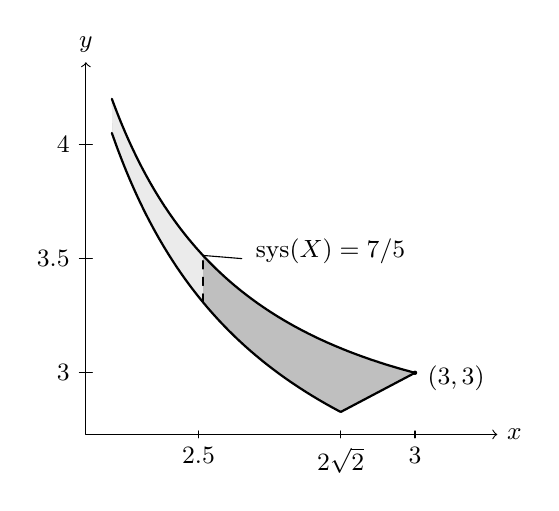
\begin{tikzpicture}[
  x=5.5cm,y=2.9cm,
  line cap=round,line join=round,
  font=\small
]
\def\xleft{2.30}
\def\xswitch{2.82842712474619}
\def\xcut{2.51033801126189}

% Visible part of the reduced region.
\def\reducedregion{
  (\xleft,{\xleft/sqrt(\xleft-2)})
  -- plot[domain=\xleft:3,samples=180]
    (\x,{\x/sqrt(\x-2)})
  -- (\xswitch,\xswitch)
  -- plot[domain=\xswitch:\xleft,samples=180]
    (\x,{2*\x/sqrt(\x*\x-4)})
  -- cycle
}

\begin{scope}
  \clip \reducedregion;
  \fill[black!25] (2.2,2.7) rectangle (3.2,4.4);
  \fill[black!8] (2.2,2.7) rectangle (\xcut,4.4);
\end{scope}

% Reduced boundaries.
\draw[thick,domain=\xleft:3,samples=180]
  plot (\x,{\x/sqrt(\x-2)});
\draw[thick] (\xswitch,\xswitch)--(3,3);
\draw[thick,domain=\xleft:\xswitch,samples=180]
  plot (\x,{2*\x/sqrt(\x*\x-4)});

% Systole cutoff.
\draw[dashed]
  (\xcut,{2*\xcut/sqrt(\xcut*\xcut-4)})
  -- (\xcut,{\xcut/sqrt(\xcut-2)});
\node[anchor=west] at (2.61,3.53) {$\operatorname{sys}(X)=7/5$};
\draw[thin] (2.60,3.50)
  -- (\xcut,{\xcut/sqrt(\xcut-2)});

% Axes; the cusp continues beyond the left edge of the view.
\draw[->] (2.24,2.73)--(3.19,2.73) node[right] {$x$};
\draw[->] (2.24,2.73)--(2.24,4.36) node[above] {$y$};
\draw (\xswitch,2.715)--(\xswitch,2.745);
\node[below] at (\xswitch,2.715) {$2\sqrt2$};
\foreach \tick in {2.5,3}{
  \draw (\tick,2.715)--(\tick,2.745);
  \node[below] at (\tick,2.715) {$\tick$};
}
\foreach \tick in {3,3.5,4}{
  \draw (2.225,\tick)--(2.255,\tick);
  \node[left] at (2.225,\tick) {$\tick$};
}

\fill (3,3) circle[radius=0.8pt];
\node[anchor=west,inner sep=2pt] at (3.015,2.975) {$(3,3)$};
\end{tikzpicture}
\par\small (a)
\end{minipage}%
\hfill
\begin{minipage}[b]{0.48\textwidth}
\centering
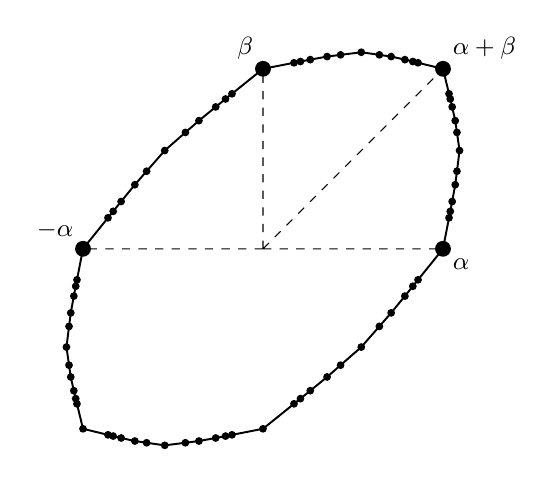
\begin{tikzpicture}[scale=4.4,font=\small]

\def\fareyplot{
(0.519522,0.000000)
(0.536938,0.089490)
(0.540555,0.108111)
(0.546015,0.136504)
(0.554821,0.184940)
(0.559813,0.223925)
(0.567296,0.283648)
(0.559813,0.335888)
(0.554821,0.369881)
(0.546015,0.409511)
(0.540555,0.432444)
(0.536938,0.447449)
(0.519522,0.519522)
(0.447449,0.536938)
(0.432444,0.540555)
(0.409511,0.546015)
(0.369881,0.554821)
(0.335888,0.559813)
(0.283648,0.567296)
(0.223925,0.559813)
(0.184940,0.554821)
(0.136504,0.546015)
(0.108111,0.540555)
(0.089490,0.536938)
(0.000000,0.519522)
(-0.089490,0.447449)
(-0.108111,0.432444)
(-0.136504,0.409511)
(-0.184940,0.369881)
(-0.223925,0.335888)
(-0.283648,0.283648)
(-0.335888,0.223925)
(-0.369881,0.184940)
(-0.409511,0.136504)
(-0.432444,0.108111)
(-0.447449,0.089490)
(-0.519522,0.000000)
}

\draw[line width=0.7pt] plot coordinates {\fareyplot};
\begin{scope}[rotate=180]
\draw[line width=0.7pt] plot coordinates {\fareyplot};
\end{scope}

\foreach \x/\y in {
0.519522/0.000000,
0.536938/0.089490,
0.540555/0.108111,
0.546015/0.136504,
0.554821/0.184940,
0.559813/0.223925,
0.567296/0.283648,
0.559813/0.335888,
0.554821/0.369881,
0.546015/0.409511,
0.540555/0.432444,
0.536938/0.447449,
0.519522/0.519522,
0.447449/0.536938,
0.432444/0.540555,
0.409511/0.546015,
0.369881/0.554821,
0.335888/0.559813,
0.283648/0.567296,
0.223925/0.559813,
0.184940/0.554821,
0.136504/0.546015,
0.108111/0.540555,
0.089490/0.536938,
0.000000/0.519522,
-0.089490/0.447449,
-0.108111/0.432444,
-0.136504/0.409511,
-0.184940/0.369881,
-0.223925/0.335888,
-0.283648/0.283648,
-0.335888/0.223925,
-0.369881/0.184940,
-0.409511/0.136504,
-0.432444/0.108111,
-0.447449/0.089490,
-0.519522/0.000000
}
{
\fill (\x,\y) circle (0.32pt);
}
\begin{scope}[rotate=180]
\foreach \x/\y in {
0.519522/0.000000,
0.536938/0.089490,
0.540555/0.108111,
0.546015/0.136504,
0.554821/0.184940,
0.559813/0.223925,
0.567296/0.283648,
0.559813/0.335888,
0.554821/0.369881,
0.546015/0.409511,
0.540555/0.432444,
0.536938/0.447449,
0.519522/0.519522,
0.447449/0.536938,
0.432444/0.540555,
0.409511/0.546015,
0.369881/0.554821,
0.335888/0.559813,
0.283648/0.567296,
0.223925/0.559813,
0.184940/0.554821,
0.136504/0.546015,
0.108111/0.540555,
0.089490/0.536938,
0.000000/0.519522,
-0.089490/0.447449,
-0.108111/0.432444,
-0.136504/0.409511,
-0.184940/0.369881,
-0.223925/0.335888,
-0.283648/0.283648,
-0.335888/0.223925,
-0.369881/0.184940,
-0.409511/0.136504,
-0.432444/0.108111,
-0.447449/0.089490,
-0.519522/0.000000
}
{
\fill (\x,\y) circle (0.32pt);
}
\end{scope}

% The four boundary directions of the three initial sectors.
\draw[dashed]
(0,0)--(0.519522,0)
(0,0)--(0.519522,0.519522)
(0,0)--(0,0.519522)
(0,0)--(-0.519522,0);

\fill (0.519522,0) circle (0.65pt);
\fill (0.519522,0.519522) circle (0.65pt);
\fill (0,0.519522) circle (0.65pt);
\fill (-0.519522,0) circle (0.65pt);

\node[below right] at (0.519522,0) {$\alpha$};
\node[above right] at (0.519522,0.519522) {$\alpha+\beta$};
\node[above left] at (0,0.519522) {$\beta$};
\node[above left] at (-0.519522,0) {$-\alpha$};

\end{tikzpicture}
\par\small (b)
\end{minipage}
\caption{(a) Reduced trace coordinates. The dashed line marks
$\sys(X)=7/5$, and the cusp has $y\to+\infty$ as $x\to2^+$.
(b) The Farey polygon $P_6(\Xmod)$ used in the area comparison
for $\sys(X)\geq7/5$.}
\label{fig:area-comparison}
\end{figure}
The polygon $P_6$ is small enough for an explicit comparison and
approximates the norm ball closely enough to control the omitted
area $$(\A-\A_6)(X):=\A(X)-\A_6(X).$$ 
Since $P_6(X)\subsetneq\B_X$, the omitted area
$(\A-\A_6)(X)$ is positive. We use the identity
\begin{equation}
\label{eq:area-comparison-split}
\A(X)-\A(\Xmod)
=\bigl[\A_6(X)-\A_6(\Xmod)\bigr]
+\bigl[(\A-\A_6)(X)-(\A-\A_6)(\Xmod)\bigr],
\end{equation}
where the first bracket is the change in polygon area and the
second is the change in omitted area. For nonmodular surfaces
with $\sys(X)\geq7/5$, we show that the polygon area increases
by more than the possible decrease in the omitted area.
For $\sys(X)<7/5$, we estimate the full area directly.

Cyclic symmetry is central to the local comparison.
The permutation $(x,y,z)\mapsto(y,z,x)$ fixes the modular point.
For every twice continuously differentiable function invariant under
this permutation, Lemma~\ref{lem:symmetry-at-modular} gives, in
local coordinates $(x,y)$,
$$
\nabla F(3,3)=0,
\qquad
\Hess F(3,3)=\kappa
\begin{pmatrix}2&1\\1&2\end{pmatrix}.
$$
Thus there is no linear term, and the quadratic term is determined
by one number. This applies to both the polygon area $\A_6$
and the omitted area $\A-\A_6$.

For the polygon area, a bound for the average squared modulus
of its complex extension on a circle controls the entire
Taylor remainder at once. The positive quadratic term then
dominates the remainder, giving
$$
\A_6(X)-\A_6(\Xmod)>\frac7{80}p_2
$$
for nonmodular $X$ in an explicit neighborhood
(Proposition~\ref{prop:uniform-p6}).
With further Taylor coefficients, the same average bound extends
the polygon comparison beyond this neighborhood.
The systole cutoff separates the two comparisons
(Figure~\ref{fig:area-comparison}(a)).
\begin{itemize}
\item
For a nonmodular torus with $\sys(X)\geq7/5$, the polygon area
increases by more than $19p_2/1000$. The omitted area can decrease by at most
$p_2/500$ by Proposition~\ref{prop:omitted-area-comparison}.
Proposition~\ref{prop:global-polygon-comparison} therefore gives
$$
\A(X)-\A(\Xmod)>\frac{17}{1000}p_2>\frac1{80}p_2.
$$

\item
If $\sys(X)<7/5$, then curves winding around a shortest
geodesic give a direct lower bound for the full area. Proposition \ref{prop:modular-upper-new} and
Theorem~\ref{thm:pure-cusp} yield
$$
\A(X)-\A(\Xmod)>\frac1{1000}.
$$
\end{itemize}
These comparisons give the explicit regional bound and prove
Theorem~\ref{thm:global-area}. For Theorem~\ref{thm:quantitative-area},
Corollary~\ref{cor:modular-minimum} gives the quadratic increase
near the modular torus, while the curves winding around a systole
give the expansion as $s_X\to0$.
In each limit, the ratio of the area gap to
$p_2e^{\sqrt{3p_2/2}}/(1+p_2)^{3/2}$ tends to a positive constant.
After excluding a small neighborhood of the modular point and
all sufficiently small systoles, the remaining reduced triples
form a compact set. On this set, the ratio is continuous and
positive by Theorem~\ref{thm:global-area}, so it has positive
lower and finite upper bounds. Together, these bounds prove
the global comparison.

\subsection{Further directions}\label{sec:Further}

Our area theorem raises questions about the dual norm-ball area,
the Mahler product, and their critical points.
We also consider an interpolation between $\A^{-1/2}$ and the
systole, and ask whether the primal and dual areas determine
the torus up to isometry. We then discuss generalized Markoff
equations and surfaces of higher complexity.

\paragraph{Dual area and the Mahler product.}
Using the standard inner product,
we identify the dual space $(\R^2)^*$ with $\R^2$. The dual norm and its unit ball
are defined by
$$
\|\lambda\|_{X,*}=\sup_{v\in\B_X}|\langle \lambda,v\rangle|,\qquad \B_X^*=\{\lambda\in\R^2:\|\lambda\|_{X,*}\leq1\}.
$$
See Figure~\ref{fig:dual-introduction}, reproduced from
\cite[Figure~3]{DLN}. For background on stable norms and their duals, see
\cite{Federer1974,BangertKatz}. 
\begin{figure}[ht]
\centering
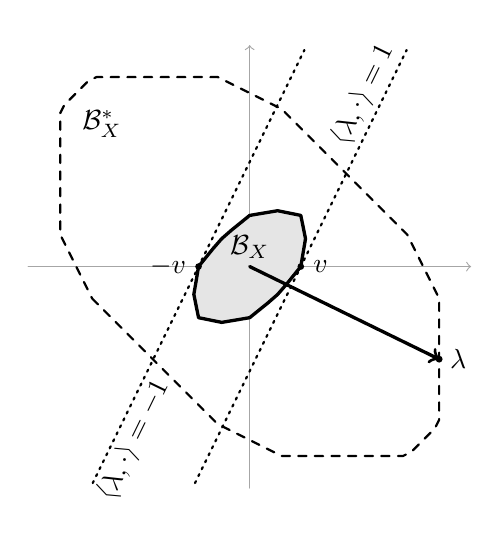
\begin{tikzpicture}[x=1.25cm,y=1.25cm,line cap=round,line join=round]
  % One common coordinate plane and one common Euclidean scale.
  \draw[->,black!35] (-2.25,0)--(2.25,0);
  \draw[->,black!35] (0,-2.25)--(0,2.25);

  % Dual body.
  \draw[thick,dashed] plot coordinates {
    (-1.600647,-0.324200) (-0.324200,-1.600647)
    (0.324200,-1.924847) (1.557457,-1.924847)
    (1.643837,-1.881657) (1.881657,-1.643837)
    (1.924847,-1.557457) (1.924847,-0.324200)
    (1.600647,0.324200) (0.324200,1.600647)
    (-0.324200,1.924847) (-1.557457,1.924847)
    (-1.643837,1.881657) (-1.881657,1.643837)
    (-1.924847,1.557457) (-1.924847,0.324200)
  } -- cycle;

  % Primal McShane--Rivin unit ball.
  \fill[black!10] plot coordinates {
    (-0.567296,-0.283648) (-0.519522,-0.519522)
    (-0.283648,-0.567296) (-0.000000,-0.519522)
    (0.184940,-0.369881) (0.283648,-0.283648)
    (0.369881,-0.184940) (0.519522,0.000000)
    (0.567296,0.283648) (0.519522,0.519522)
    (0.283648,0.567296) (0.000000,0.519522)
    (-0.184940,0.369881) (-0.283648,0.283648)
    (-0.369881,0.184940) (-0.519522,-0.000000)
  } -- cycle;
  \draw[very thick] plot coordinates {
    (-0.567296,-0.283648) (-0.519522,-0.519522)
    (-0.283648,-0.567296) (-0.000000,-0.519522)
    (0.184940,-0.369881) (0.283648,-0.283648)
    (0.369881,-0.184940) (0.519522,0.000000)
    (0.567296,0.283648) (0.519522,0.519522)
    (0.283648,0.567296) (0.000000,0.519522)
    (-0.184940,0.369881) (-0.283648,0.283648)
    (-0.369881,0.184940) (-0.519522,-0.000000)
  } -- cycle;

  % A boundary vector v of the dual body and its two supporting lines.
  \draw[->,very thick] (0,0)--(1.924847,-0.940829)
    node[pos=1,right] {$\lambda$};
  \fill (1.924847,-0.940829) circle (1.25pt);

  \draw[dotted,thick] (-0.555797,-2.200000)--(1.594840,2.200000);
  \draw[dotted,thick] (-1.594840,-2.200000)--(0.555797,2.200000);

  \fill (0.519522,0) circle (1.2pt) node[right=1pt] {$v$};
  \fill (-0.519522,0) circle (1.2pt) node[left=1pt] {$-v$};

  \node[rotate=64,anchor=south] at (1.37,1.64)
    {$\langle \lambda,\cdot\rangle=1$};
  \node[rotate=64,anchor=north] at (-1.39,-1.66)
    {$\langle \lambda,\cdot\rangle=-1$};

  \node at (-0.0,0.20) {$\B_X$};
  \node at (-1.50,1.45) {$\B_X^*$};
\end{tikzpicture}
\caption{The unit ball $\B_X$ and its dual body $\B_X^*$, where $X$ is the modular torus.}
\label{fig:dual-introduction}
\end{figure}
Doan, Li, and Nguyen proved the identity
\cite[Theorem~1.3]{DLN}
$$
\mathcal A^*(X)
=4\sum_\gamma\ell_X(\gamma)\log\coth\frac{\ell_X(\gamma)}2,
$$
where $\A^*(X):=\Area(\B_X^*)$ and the sum runs over unoriented essential simple closed geodesics.
The \emph{Mahler product}
$$
\operatorname{Mah}(X)=\A(X)\A^*(X)
$$
is invariant under invertible linear changes of coordinates and
rescaling of the norm, and therefore measures the shape of the ball. The planar Mahler inequality \cite{Mahler,Reisner} and the
Blaschke--Santal\'o inequality \cite{MeyerPajor} give
$8\leq \operatorname{Mah}(X)\leq\pi^2$, with equality precisely for parallelograms
and ellipses, respectively. See
\cite{BoroczkyMakaiMeyerReisner,Ivaki} for planar stability
estimates and \cite{Schneider,FradeliziMeyerZvavitch} for background.
The lower bound is the planar case of the symmetric Mahler
conjecture on minimum volume products in arbitrary
dimension.\footnote{A recent preprint released by OpenAI
\cite{OpenAIMahler} reports a proof of the symmetric Mahler
conjecture in every dimension.} However, these bounds are strict in the family of hyperbolic once-punctured tori, since
$\B_X$ is strictly convex and has corners at rational directions
\cite{McShaneRivinTori,DLN}. We propose
the following conjecture for the maximum Mahler product
within this family.

\begin{conjecture}\footnote{After receiving our preliminary draft, Ying Zhang
began working on Conjecture~\ref{conj:mahler-maximum}
and later reported a joint proof with Hu Tan~\cite{TanZhang26}, based on our
method. They also show that the Mahler
product tends to $8$ as $s_X\to0$.}\label{conj:mahler-maximum}
Every complete finite-area hyperbolic once-punctured torus $X$ satisfies
$$
\operatorname{Mah}(X)\leq \operatorname{Mah}(\Xmod),
$$
with equality exactly when $X$ and $\Xmod$ are isometric.
\end{conjecture}
Together with Theorem~\ref{thm:global-area}, Conjecture \ref{conj:mahler-maximum} would give
$$
\A^*(X)
=\frac{\operatorname{Mah}(X)}{\A(X)}
\leq\frac{\operatorname{Mah}(\Xmod)}{\A(\Xmod)}
=\A^*(\Xmod),
$$
with strict inequality for every nonmodular torus, thus $\Xmod$
uniquely minimizes $\A$, $-\A^*$, and $-\operatorname{Mah}$.
The dual area also governs an intersection-counting problem. Let $\alpha,\beta$ range over unoriented essential simple closed
geodesics, and let $i(\alpha,\beta)$ denote their geometric
intersection number. For primitive homology vectors $(p,q)$
and $b$ representing them,
$i(\alpha,\beta)=|\langle(-q,p),b\rangle|$.
Thus, by continuity, the intersection bound below is equivalent
to $(-q,p)\in L\B_X^*$.
The rotation $(p,q)\mapsto(-q,p)$ preserves the integer lattice
and area, so the lattice argument used in \eqref{eq:Counting} gives
\begin{equation}\label{eq:ICounting}
    \#\{\alpha:i(\alpha,\beta)\leq L\ell_X(\beta)
          \text{ for every }\beta\}=\frac3{\pi^2}\A^*(X)L^2+O_X(L\log L).
\end{equation}
The modular torus would therefore have more curves satisfying this
intersection bound than each fixed nonmodular torus for all
sufficiently large $L$.
The two areas also govern lattice counting for the Thurston metric.
For the once-punctured torus, the stable norm gives the following
explicit consequence of the general lattice-counting theorem of
Gorodnik and Nevo \cite{GorodnikNevo}.

\begin{proposition}[Thurston lattice counting]\label{prop:thurston-counting}
Let $X,Y$ be complete finite-area hyperbolic once-punctured tori,
and let $\operatorname{Mod}(S)$ be the orientation-preserving
mapping class group. Set
$$
N_{X,Y}(R)=
\#\{\phi\in\operatorname{Mod}(S):
d_{\mathrm{Th}}(X,\phi Y)\leq R\}.
$$
Then
\begin{equation}\label{eq:thurston-torus-counting}
N_{X,Y}(R)=
\frac{6}{\pi^2}\A^*(X)\A(Y)e^{2R}
+o_{X,Y}(e^{2R}).
\end{equation}
In particular,
$$
N_{X,X}(R)\sim
\frac{6}{\pi^2}\operatorname{Mah}(X)e^{2R}.
$$
\end{proposition}
For fixed $X$, Theorem~\ref{thm:global-area} therefore gives
$N_{X,\Xmod}(R)<N_{X,Y}(R)$ for each fixed nonmodular $Y$
and all sufficiently large $R$.
When $X=Y$, Conjecture~\ref{conj:mahler-maximum} predicts that
the modular torus maximizes the leading coefficient.
\begin{proof}[Proof sketch of Proposition \ref{prop:thurston-counting}]
The homology action identifies $\operatorname{Mod}(S)$ with
$\operatorname{SL}_2(\Z)$ \cite{FarbMargalit}. Both $A$ and $-A$
are counted, although they act identically on Teichm\"uller space.
Thurston's length-ratio formula
\cite[Theorem~8.5]{ThurstonMinimalStretch} reduces the count,
after matrix inversion, to integral points in
$$
\Omega_R=\{g\in\operatorname{SL}_2(\R):
g\B_X\subset e^R\B_Y\}.
$$
With Haar volume normalized so that
$\operatorname{SL}_2(\R)/\operatorname{SL}_2(\Z)$ has volume one,
$$
\operatorname{vol}(\Omega_R)
\sim\frac6{\pi^2}\A^*(X)\A(Y)e^{2R}.
$$
The verification of well-roundedness
\cite[Definition~1.1]{GorodnikNevo} is left to the reader.
The lattice-counting theorem
\cite[Theorem~1.7 and Remark~4.6(ii)]{GorodnikNevo}
then gives \eqref{eq:thurston-torus-counting}.
\end{proof}
\paragraph{Critical points and rigidity.}
Numerical computations also suggest that the square punctured
torus, represented by the trace triple $(2\sqrt2,2\sqrt2,4)$,
is a saddle point of $\A,\mathcal A^*,\operatorname{Mah}$. These extremal observations raise a broader question about the full
critical-point structure of these functions. Recall that a smooth function is \emph{Morse} if its Hessian is nondegenerate
at every critical point. Classical examples on Teichm\"uller space
include sums of geodesic lengths of curves that fill the surface\cite{Wolpert1987}.
Chen constructed $C^2$-Morse approximations to the systole on
moduli space \cite{Chen2025Morse}. For sufficiently small smoothing
parameter, these have exactly two critical points on the moduli space
of once-punctured tori: a maximum at the modular torus and a saddle
at the square punctured torus \cite[Section~8.2]{Chen2025Morse}.
Related work on the topological Morse property, defined using
homeomorphic local coordinates \cite{Morse1959}, concerns systoles
\cite{SchmutzSchaller1999,Akrout2003} and the diameter
\cite{IrmerSaha2026}.

\begin{question}\label{qu:morse-invariants}
Are $\A$, $-\A^*$, and $-\operatorname{Mah}$ Morse functions
on the Teichm\"uller space of the once-punctured torus,
each having, modulo the mapping class group, exactly two
critical points: a minimum at the modular torus and a saddle
at the square punctured torus?
\end{question}
Corollary~\ref{cor:modular-minimum} establishes the nondegenerate
minimum at the modular torus for $\A$.

The norm-ball area governs the growth of simple geodesics at
large lengths, while the systole records the shortest length.
To incorporate information from all length scales, following
Babenko and Massart's use of zeta functions for stable norms
\cite{BabenkoMassart2017}, define, for $p>2$,
$$
F_p(X)=
\left(
(p-2)\zeta(p)\sum_\gamma \ell_X(\gamma)^{-p}
\right)^{-1/p},
$$
where the sum runs over unoriented essential simple closed
geodesics and $\zeta$ is the Riemann zeta function.
The sum weights each simple geodesic by an inverse power of its
length, giving increasing emphasis to the shortest geodesics
as $p$ grows.
The factor $\zeta(p)$ accounts for positive multiples of
primitive homology classes.
The counting asymptotic \eqref{eq:Counting} and domination by
the shortest lengths give, for every fixed $X$,
$$
\lim_{p\downarrow2}F_p(X)=\A(X)^{-1/2},\qquad
\lim_{p\to\infty}F_p(X)=\sys(X).
$$
This interpolation motivates the following analogue of
Chen's critical-point description.
\begin{question}\label{qu:morse-interpolation}
For every $p>2$, is $F_p$ a Morse function on the
Teichm\"uller space of the once-punctured torus,
with exactly two critical orbits under the mapping class group:
a maximum at the modular torus and a saddle at the
square punctured torus?
\end{question}

The counting formulas \eqref{eq:Counting} and \eqref{eq:ICounting}
associate two leading coefficients to each torus. Numerical
computations suggest that these two coefficients together
determine its isometry class.
\begin{question}\label{conj:area-rigidity}
Is a complete finite-area hyperbolic once-punctured torus determined
up to isometry by the pair $(\A,\mathcal A^*)$?
\end{question}
To answer this question, it would suffice to show that, for every
$c>\A(\Xmod)$, the level set $\A=c$ in the reduced region is a single
arc along which $\mathcal A^*(X)$ is strictly monotone.
Geometrically, this would mean that the intersection counting
coefficient distinguishes tori with the same ordinary counting
coefficient. The Farey area expansion and the dual-area identity
above provide formulas for studying this monotonicity.
The main difficulty is to control the derivatives throughout
the reduced region, especially as $x\to2$, where the systole
tends to zero.

\paragraph{Higher complexity.}
For a complete finite-area hyperbolic surface of type $(g,n)$,
put $D=6g-6+2n>0$. The analogue of the norm-ball area is
the Mirzakhani function
$$
m(X)=\mu_{\mathrm{Th}}
\{\lambda\in\mathcal{ML}_{g,n}:\ell_X(\lambda)\leq1\}.
$$
Mirzakhani's counting theorem gives
$N_X(L)\sim c_{g,n}m(X)L^D$, where $c_{g,n}>0$ depends
only on the topological type \cite{MirzakhaniGrowth}. The interpolation above extends by defining, for $p>D$,
$$
G_p(X)=
\left(
\frac{p-D}{D c_{g,n}}
\sum_\gamma\ell_X(\gamma)^{-p}
\right)^{-1/p}.
$$
Partial summation and domination by the shortest
lengths give, for every fixed $X$,
$$
\begin{aligned}
\lim_{p\downarrow D}G_p(X)&=m(X)^{-1/D},\qquad
\lim_{p\to\infty}G_p(X)&=\sys(X).
\end{aligned}
$$
One may ask for which $p>D$ these functions are Morse and
how their critical points depend on $p$.
Up to an additive constant independent of $X$,
$$
\log G_p(X)
=-\frac1p\log\sum_\gamma e^{-p\log\ell_X(\gamma)}.
$$
This suggests adapting Chen's analysis to logarithmic length
functions \cite{Chen2025Morse}.

The dual-area question requires a construction on measured
lamination space. On closed surfaces of higher genus,
separating curves are homologically trivial, so the homological
stable norm does not capture all simple curves.
Moreover, $\mathcal{ML}_{g,n}$ has no canonical global
vector-space structure on which to take a dual space.
The intersection-counting interpretation \eqref{eq:ICounting} leads to the set
$$
\{\lambda\in\mathcal{ML}_{g,n}:
i(\lambda,\mu)\leq\ell_X(\mu)
\text{ for every }\mu\in\mathcal{ML}_{g,n}\}.
$$
This is the unit ball considered by Rafi and Souto
\cite[Equation~(1.2)]{RafiSouto}.
Its Thurston volume, denoted by $m^*(X)$, appears in their lattice-counting theorem
for the Thurston metric on closed surfaces
\cite[Theorem~1.1]{RafiSouto}.
Erlandsson and Souto extend this lattice-counting theorem to
punctured surfaces of genus at least two
\cite[Theorem~12.6 and Exercise~12.6]{ErlandssonSoutoBook}.
Taking the same surface as the base point and orbit
representative gives a counting interpretation to
$m(X)m^*(X)$, extending the torus interpretation
in Proposition~\ref{prop:thurston-counting}.
This motivates studying the extrema
and Morse properties of $m$, $m^*$, and $mm^*$.
\paragraph{Organization of the paper.}
Sections~\ref{sec:coordinates} and~\ref{sec:shared-estimates}
develop the coordinates and estimates used in the two regional
comparisons in Sections~\ref{sec:large-systole} and~\ref{sec:short-systole}.
Section~\ref{sec:completion} completes the proofs of the main theorems.
Appendix~\ref{sec:cusp-growth} proves the cusp expansion.

\paragraph{Acknowledgements and declaration of AI use.} We thank Greg McShane and Igor Rivin for their influential work.
The ideas of subdividing the reduced region and estimating area
changes along lines through the modular point
(Subsections~\ref{sec:taylor-expansion} and
\ref{sec:omitted-area}) arose in part from discussions
with Ser Peow Tan during the last-named author's visit to the
National University of Singapore in May 2026.
The last-named author thanks him for these helpful discussions and for
encouraging us to pursue the conjecture. The background and some estimates were influenced by the recent work \cite{DLN} of the last-named author with Xiaobin Li and Van Nguyen.
ChatGPT (OpenAI) assisted with technical estimates, numerical
experiments, and literature searches.
The authors meticulously wrote and revised the paper, devoting
substantial effort to simplifying several long and tedious
calculations and making them accessible to a broader readership.
The second-named author is supported by the NUS President Graduate Fellowship. 

\section{Trace coordinates and Farey polygons}
\label{sec:coordinates}

This section introduces the notations, coordinates, area formulas,
and differential tools used in the proof.
\subsection{Trace coordinates and reduction}
Oriented essential simple closed curves on the once-punctured torus $S$ correspond to nonzero primitive classes
in $H_1(S;\Z)$.
Two primitive classes $u,v$ are Farey neighbors exactly when their
algebraic intersection number has absolute value one. Fix a complete finite-area hyperbolic structure $X$ on $S$ and let $\|\cdot\|_X$ be the stable norm on
$H_1(S;\R)$. For a primitive class $u$, define its trace by
$$
x_u=2\cosh\frac{\|u\|_X}{2}.
$$
For every pair of Farey neighbors $u,v$, the traces
$x_u,x_v,x_{u+v}$ satisfy the Markoff equation
\begin{equation}
\label{eq:markoff}
x_u^2+x_v^2+x_{u+v}^2=x_ux_vx_{u+v},
\end{equation}
and the two traces across the corresponding Farey edge satisfy
\begin{equation}
\label{eq:vieta}
x_{u+v}+x_{u-v}=x_ux_v.
\end{equation}
See \cite{Bowditch}. Thus crossing the edge replaces the Farey triangle
$(u,v,u-v)$ by $(u,v,u+v)$ and induces the Vieta move
$$
x_{u-v}\longmapsto x_ux_v-x_{u-v}=x_{u+v}.
$$
The positive solutions of the Markoff equation give the usual trace
coordinates for marked complete hyperbolic punctured tori, see
\cite[Theorem~4.1.2 and Section~4.4]{GoldmanTrace}. We call a solution
$(x,y,z)\in(2,\infty)^3$ a \emph{positive Markoff triple}.
For $(x,y,z)=(x_u,x_v,x_{u+v})$, replacing the ordered basis
$(u,v)$ by $(v,-u-v)$ gives the three classes $v,-u-v,-u$.
Since $x_{-w}=x_w$, this change induces the cyclic permutation
\begin{equation}
\label{eq:cyclic-trace-permutation}
\rho(x,y,z)=(y,z,x).
\end{equation}
For fixed $x,y$, solving the Markoff equation for $z$ gives
$$
z_\pm(x,y)
=
\frac{xy\pm\sqrt{\mathscr D(x,y)}}2,
\qquad
\mathscr D(x,y):=x^2y^2-4x^2-4y^2.
$$
For every real Markoff triple $(x,y,z)$,
$$
\mathscr D(x,y)
=
x^2y^2-4xyz+4z^2
=
(xy-2z)^2
\geq0.
$$
Thus the two branches $z_\pm$ are distinct and real analytic wherever
$x,y>2$ and $\mathscr D(x,y)>0$. They coincide exactly on
$\mathscr D=0$, where
$$
z_+(x,y)=z_-(x,y)=\frac{xy}{2}.
$$
A positive Markoff triple $(x,y,z)$ is \emph{reduced} if
$$2<x\leq y\leq z\leq\frac{xy}{2},$$
as illustrated in Figure~\ref{fig:area-comparison}(a). Thus, for a
reduced triple,
$$
z=z_-(x,y).
$$
A Farey triangle is called a \emph{sink} if none of its three
adjacent Vieta moves decreases the trace it replaces.

\begin{proposition}[Markoff reduction]
\label{prop:markoff-reduction}
Every positive Markoff triple is equivalent under permutations and
Vieta moves to a reduced triple. If $(x,y,z)$ is a reduced triple
representing $X$, then
$$
x=2\cosh\frac{\sys(X)}2,
\qquad
x\leq3,
\qquad
y\leq\frac{x}{\sqrt{x-2}}.
$$
\end{proposition}

\begin{proof}
Associate $X$ with its Markoff map on the Farey tree. The reduction
argument \cite[Section~3]{Bowditch} gives a sink triangle.
Order its traces as $x\leq y\leq z$. Then $z\leq xy-z$, so the triple is reduced.

Conversely, every Vieta move from a reduced triple produces a
trace at least as large as $z$. Consider an arbitrary path without
reversing a move. At each later step
$
(U,V,W)\longmapsto(U,V,UV-W),
$
one of $U,V$ is the trace produced at the previous step.
Inductively, it is at least as large as $W$, so
$$
UV-W\geq UV-\max(U,V)>\max(U,V),
$$
since $U,V>2$. Thus $x$ is the smallest trace, so
$x=2\cosh(\sys(X)/2)$. Finally, \eqref{eq:markoff} and reducedness give
$$
x^2+y^2=z(xy-z)\geq y(xy-y)=(x-1)y^2,
$$
since $t(xy-t)$ is increasing on $(-\infty,xy/2]$ and
$
y\leq z\leq xy/2.
$
Therefore
$
y\leq x/\sqrt{x-2}.
$
Since $y\geq x$, it follows that $x\leq3$.
\end{proof}

For the local estimates near the modular torus, we use the branch
$z=z_-(x,y)$ near $(3,3)$. The discriminant is positive there since
$\mathscr D(3,3)=9$. Write $\A(x,y)$ for the area of the torus
with trace triple $(x,y,z_-(x,y))$. This function is real analytic
\cite[Section~3, Corollary~1]{McShaneRivinTori}.
See also \cite[slide~30]{Bonahon2018}.

\subsection{The exact Farey area expansion}
\label{sec:farey-area}

To construct the Farey polygons for a surface $X$, choose a reduced
trace triple $(x,y,z)$ and an ordered integral basis $(\alpha,\beta)$
realizing it:
$$
(x_\alpha,x_\beta,x_{\alpha+\beta})=(x,y,z).
$$
The Farey triangle $(\alpha,\beta,\alpha+\beta)$ is a sink by
Proposition~\ref{prop:markoff-reduction}. We use it as the initial
triangle; this choice may depend on $X$.

When varying the trace triple near the modular point, we keep the
initial triangle fixed. On a neighborhood of $(3,3,3)$, its three
Vieta moves strictly increase the traces they replace. The curves
and sector heights are therefore fixed in these local coordinates.
A move away from the initial triangle is called an
\emph{outward Farey insertion}.

For each of the three initial sectors, let $(u_0,v_0)$ denote its
endpoints:
$$
(u_0,v_0)\in
\{(\alpha,\alpha+\beta),(\alpha+\beta,\beta),(\beta,-\alpha)\}.
$$
Every primitive class in this sector has a unique expression
$w=pu_0+qv_0$ with nonnegative integers $p,q$. Define its
\emph{sector height} by
$$
h(w)=p+q.
$$
Starting from these three intervals, recursively insert $u+v$
between the endpoints of each current interval $(u,v)$, replacing
it by $(u,u+v)$ and $(u+v,v)$. At each insertion, we call $u,v$
the \emph{parents} and $u+v$ their \emph{child}.
Let $\mathscr F$ be the set of all intervals occurring in this
subdivision, including the initial ones.
Heights are always measured relative to the fixed endpoints
$(u_0,v_0)$ of the initial sector containing the interval.
Thus, for every $(u,v)\in\mathscr F$,
$$
h(u+v)=h(u)+h(v).
$$
Every primitive class in the interior of an initial sector is
inserted exactly once.

For $K\geq1$, let $P_K(X)$ be the centrally symmetric inscribed polygon
whose vertices are the normalized primitive classes of sector height at
most $K$, together with their negatives, and set
$$
\A_K(X)=\Area(P_K(X)).
$$
For $K=6$ and a reduced triple, this is the polygon used in the
introduction (Figure~\ref{fig:area-comparison}(b)). In the local family, the sectors
and heights are fixed; only the geodesic lengths used to normalize
the vertices vary. Thus the same construction defines $\A_K$ for
the nearby triples used in the local estimates.

For a primitive class $u$, write
$$
L_u=\|u\|_X=2\arccosh\frac{x_u}{2}.
$$
If $u+v$ is inserted between Farey neighbors $u,v$, then the edge joining
$u/L_u$ to $v/L_v$ is replaced by the two edges through
$(u+v)/L_{u+v}$ (see Figure~\ref{fig:area-correction}). 
\begin{figure}[ht]
\centering
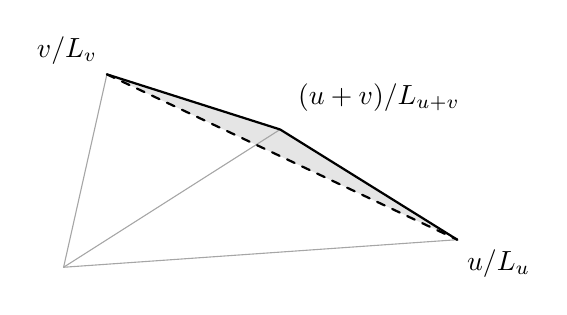
\begin{tikzpicture}[
    scale=1,
    line cap=round,
    line join=round
]

\coordinate (O) at (0,0);
\coordinate (V) at (0.55,2.45);
\coordinate (U) at (5.00,0.35);
\coordinate (W) at (2.75,1.75);

\fill[gray!20] (V)--(W)--(U)--cycle;

\draw[gray!70] (O)--(V);
\draw[gray!70] (O)--(W);
\draw[gray!70] (O)--(U);

\draw[dashed,thick] (V)--(U);
\draw[thick] (V)--(W)--(U);

\node[above left] at (V) {$v/L_v$};
\node[below right] at (U) {$u/L_u$};
\node[above right=3pt] at (W) {$(u+v)/L_{u+v}$};

\end{tikzpicture}
\caption{The area added by one Farey insertion on one side of the norm ball.}
\label{fig:area-correction}
\end{figure}

Since
$$
|\det(u,v)|=|\det(u,u+v)|=|\det(u+v,v)|=1,
$$
the shaded triangle has area
$$
\frac12\left(
\frac1{L_uL_{u+v}}
+\frac1{L_{u+v}L_v}
-\frac1{L_uL_v}
\right).
$$
Including its antipodal copy, the total area gain is
\begin{equation}
\label{eq:area-gain}
S_X(u,v)
:=
\frac1{L_uL_{u+v}}
+\frac1{L_{u+v}L_v}
-\frac1{L_uL_v}
=
\frac{L_u+L_v-L_{u+v}}{L_uL_vL_{u+v}}.
\end{equation}
This is positive by the strict triangle inequality
$L_{u+v}<L_u+L_v$ \cite[Section~2]{McShaneRivinTori}. We obtained the following expansion independently.
It also follows from O'Sullivan's formula
\cite[Proposition~6.5]{OSullivan2026}, which generalizes
Zagier's formula for the Markoff counting constant
\cite[equation~(3)]{Zagier1982}.
Specializing it to \eqref{eq:markoff}, converting half-lengths
to lengths, and summing over the three initial sectors gives
our expansion.

\begin{proposition}[Farey area expansion]
\label{prop:farey-expansion}
The polygons $P_K(X)$ are nested and
$$
\A_K(X)\nearrow\A(X).
$$
Moreover,
$$
\A_K(X)
=
\A_1(X)
+
\sum_{\substack{(u,v)\in\mathscr F\\h(u+v)\leq K}}
S_X(u,v),
$$
and hence
$$
\A(X)
=
\A_1(X)
+
\sum_{(u,v)\in\mathscr F}S_X(u,v).
$$
\end{proposition}

\begin{proof}
Increasing $K$ only adds boundary points of $\B_X$, so the polygons are
nested. Since primitive directions are dense and the norm is continuous,
$P_K(X)$ converges to $\B_X$ in the Hausdorff metric. Hence
$
\A_K(X)$ converges to $\A(X)
$
by \cite[Theorem~1.8.20]{Schneider}.
Summing $S_X(u,v)$ over all insertions of height at most $K$ gives
the finite formula, and letting $K\to\infty$ gives the expansion of $\A$.
\end{proof}

We record three facts that will be used repeatedly. First,
Proposition~\ref{prop:farey-expansion} gives the tail identity
\begin{equation}
\label{eq:farey-tail}
\A(X)-\A_K(X)
=
\sum_{\substack{(u,v)\in\mathscr F\\h(u+v)>K}}
S_X(u,v).
\end{equation}

Second, at sector height $H\geq2$, each initial sector contains exactly
$\varphi(H)$ inserted classes, where
$\varphi(H)=\#\{1\leq p<H:\gcd(p,H)=1\}$ is Euler's totient function.
Indeed, these classes correspond to primitive pairs $p,q>0$ with
$p+q=H$. Hence
\begin{equation}
\label{eq:farey-height-count}
\#\{(u,v)\in\mathscr F:h(u+v)=H\}
=3\varphi(H)\leq3(H-1).
\end{equation}

Third, for an initial trace triple $(x,y,z)$, write $\A_K(x,y,z)$ for
the polygon area $\A_K(X)$ determined by that initial Farey triangle.
Permuting its three vertices only relabels the three sectors and preserves
sector height and lattice area. Hence, for every permutation $\sigma$ of the three coordinates,
\begin{equation*}
\A_K(\sigma(x,y,z))=\A_K(x,y,z).
\end{equation*}
As for $\A$, we regard $\A_K$ as a function of the local coordinates
$(x,y)$ by writing
$$
\A_K(x,y):=\A_K(x,y,z_-(x,y)).
$$
In particular, $\A_K(3,3)=\A_K(\Xmod)$.



\subsection{Derivatives and symmetry at the modular point}
\label{sec:differential-tools}
We recall the gradient and Hessian and explain how cyclic symmetry
constrains them at the modular point.
\paragraph{Gradient and Hessian.}
For a twice continuously differentiable function $G(x,y)$, recall that
$$
\nabla G=
\begin{pmatrix}
G_x\\
G_y
\end{pmatrix},
\qquad
\Hess G=
\begin{pmatrix}
G_{xx}&G_{xy}\\
G_{xy}&G_{yy}
\end{pmatrix}.
$$
For a direction $v\in\R^2$, the directional derivative is
$$
D_vG=\nabla G\cdot v.
$$
Thus $\nabla G=0$ means that $G$ has zero first-order slope in every
direction. Suppose the segment $q+sv$, $0\leq s\leq1$, lies in the
domain of $G$. Applying Taylor's theorem \cite[Theorem~5.15]{Rudin}
to $s\mapsto G(q+sv)$ gives, for some $\theta\in(0,1)$,
\begin{equation}
\label{eq:taylor-segment}
G(q+v)-G(q)
=\nabla G(q)\cdot v+\frac12v^{\mathsf T}\Hess G(q+\theta v)v.
\end{equation}
By continuity of the Hessian, as $v\to0$ we have
\begin{equation}
\label{eq:taylor-quadratic}
G(q+v)-G(q)
=\nabla G(q)\cdot v+\frac12v^{\mathsf T}\Hess G(q)v+o(|v|^2).
\end{equation}
The notation $\Hess G(q)\geq0$ means that
$v^{\mathsf T}\Hess G(q)v\geq0$ for every vector $v$.
On a convex domain, $G$ is convex exactly when this holds at every point.
Let
$$
\Sigma
=
\{(x,y,z)\in\R^3:x^2+y^2+z^2=xyz\}
$$
be the Markoff surface, and let
$
p=(3,3,3)
$
be the modular point (see Figure~\ref{fig:markoff-surface-tangent-plane}).
The following lemma is an elementary consequence of cyclic symmetry (see \cite{Palais1979}).

\begin{lemma}[Order-three symmetry at the modular torus]
\label{lem:symmetry-at-modular}
Suppose $\widetilde F$ is twice continuously differentiable on
$\Sigma$ near $p$ and invariant under cyclic permutation of the
coordinates. On the branch $z=z_-(x,y)$, define
$$
F(x,y)=\widetilde F(x,y,z_-(x,y)).
$$
Then
$$
\nabla F(3,3)=0,
\qquad
\Hess F(3,3)
=
\kappa
\begin{pmatrix}
2&1\\
1&2
\end{pmatrix}
$$
for some real $\kappa$.
\end{lemma}

\begin{proof}
Since $\nabla(x^2+y^2+z^2-xyz)(p)=(-3,-3,-3)$,
the tangent plane is $T_p\Sigma=\{a+b+c=0\}$.
Translating it
to $p$ gives the affine tangent plane
$
p+T_p\Sigma
$
as shown in Figure~\ref{fig:markoff-surface-tangent-plane}.


\begin{figure}[ht]
\centering

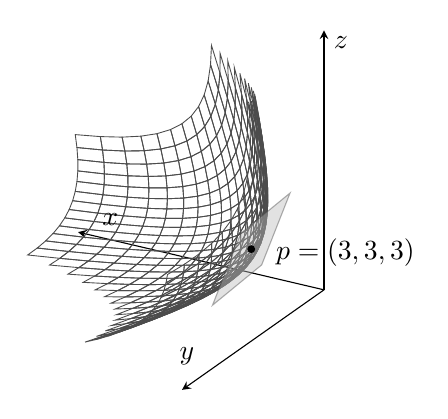
\begin{tikzpicture}
\begin{axis}[
    width=10.5cm,
    height=8.5cm,
    view={210}{24},
    axis lines=center,
    axis equal image,
    xlabel={$x$},
    ylabel={$y$},
    zlabel={$z$},
    xmin=2.1, xmax=6.9,
    ymin=2.1, ymax=6.9,
    zmin=2.1, zmax=6.9,
    ticks=none,
    enlargelimits=false,
    clip=false,
    unbounded coords=jump,
]

\def\Rho{0.50}
\def\PlaneRho{0.16}

% Positive Markoff surface.
% Put w=-u-v and
% S=e^{2u}+e^{2v}+e^{2w}.
% Then
% (x,y,z)=(e^uS,e^vS,e^wS)
% satisfies x^2+y^2+z^2=xyz.

\addplot3[
    mesh,
    color=black!70,
    line width=0.32pt,
    samples=27,
    samples y=27,
    domain=-\Rho:\Rho,
    y domain=-\Rho:\Rho,
]
(
{
ifthenelse(
max(abs(x),max(abs(y),abs(x+y))) <= \Rho,
exp(x)*(exp(2*x)+exp(2*y)+exp(-2*x-2*y)),
nan
)
},
{
ifthenelse(
max(abs(x),max(abs(y),abs(x+y))) <= \Rho,
exp(y)*(exp(2*x)+exp(2*y)+exp(-2*x-2*y)),
nan
)
},
{
ifthenelse(
max(abs(x),max(abs(y),abs(x+y))) <= \Rho,
exp(-x-y)*(exp(2*x)+exp(2*y)+exp(-2*x-2*y)),
nan
)
}
);

% Affine tangent plane p+T_p Sigma: x+y+z=9.
\addplot3[
    surf,
    shader=flat,
    draw=gray!55!black,
    fill=gray!55,
    opacity=0.42,
    samples=2,
    samples y=2,
    variable=u,
    variable y=v,
    domain=-\PlaneRho:\PlaneRho,
    y domain=-\PlaneRho:\PlaneRho,
]
(
    {3+3*u},
    {3+3*v},
    {3-3*u-3*v}
);

% Modular point.
\addplot3[
    only marks,
    mark=*,
    mark size=1.2pt,
    black
]
coordinates {(3,3,3)};

\node[
    anchor=west,
    inner sep=2pt
]
at (axis cs:2.62,3.02,3.02)
{$p=(3,3,3)$};

\end{axis}
\end{tikzpicture}

\caption{
The Markoff surface near $p=(3,3,3)$ and its affine tangent
plane.
}
\label{fig:markoff-surface-tangent-plane}
\end{figure}

By \eqref{eq:cyclic-trace-permutation}, $\rho$ fixes $p=(3,3,3)$
and acts on $T_p\Sigma$ as a rotation through $120^\circ$.
Hence the three vectors $\xi,\rho\xi,\rho^2\xi$ sum to zero for every $\xi\in T_p\Sigma$.
Cyclic invariance makes the directional derivatives along these
vectors equal, so linearity gives
$$
3D_\xi\widetilde F(p)
=
D_{\xi+\rho\xi+\rho^2\xi}\widetilde F(p)
=
0.
$$
Thus every tangential derivative vanishes, and the chain rule yields
$\nabla F(3,3)=0$.

For the second derivatives, let $\gamma$ be a twice continuously
differentiable curve in $\Sigma$ with $\gamma(0)=p$ and
$\gamma'(0)=\xi=(a,b,-a-b)$. Since $\nabla F(3,3)=0$,
the acceleration terms vanish in the chain rule, giving
$$
\frac{d^2}{dt^2}\widetilde F(\gamma(t))\bigg|_{t=0}
=
F_{xx}(3,3)a^2+2F_{xy}(3,3)ab+F_{yy}(3,3)b^2.
$$
This depends only on $\xi$, so it defines a quadratic form
$Q$ on $T_p\Sigma$. Cyclic invariance gives $Q(\rho\xi)=Q(\xi)$. If $Q$ is not constant on the Euclidean unit circle in $T_p\Sigma$,
then its maximum is attained at exactly two opposite points.
A $120^\circ$ rotation cannot preserve this pair, so cyclic
invariance forces $Q$ to be constant on the unit circle. By homogeneity,
$$
Q(\xi)=\kappa|\xi|^2
=\kappa\bigl(a^2+b^2+(a+b)^2\bigr).
$$
Comparing coefficients yields the formula for 
$
\Hess F(3,3)
$ as desired.
\end{proof}

\section{Farey polygon estimates}
\label{sec:shared-estimates}

To apply \eqref{eq:area-comparison-split}, we estimate the added
areas $S_X(u,v)$, give the polygon's area formula, and estimate the modular
area and its omitted terms. We then compute the Taylor coefficients,
control the remainder, and obtain polygon bounds near the modular point.


\subsection{Length and added-area estimates}
\label{sec:local}
The area gain in \eqref{eq:area-gain} involves the lengths of both
parents and their child. To estimate the terms of the Farey area
expansion, we eliminate the child length using the Markoff equation.
For an edge with endpoint traces $x_u,x_v$, the two opposite traces
are the roots of
\begin{equation}
\label{eq:2trace}
T^2-x_ux_vT+x_u^2+x_v^2=0.
\end{equation}
By Proposition~\ref{prop:markoff-reduction}, every outward insertion
from a reduced triangle uses the larger root. Substituting
$x_w=2\cosh(L_w/2)$ gives the corresponding child length
\begin{equation}
\label{eq:child-length}
\cosh\frac{L_{u+v}}{2}
=
\cosh\frac{L_u}{2}\cosh\frac{L_v}{2}
+
\sqrt{\sinh^2\frac{L_u}{2}\sinh^2\frac{L_v}{2}-1}.
\end{equation}

We now treat the parent lengths as independent variables on the domain
where the square root is real, namely
\begin{equation}
\label{eq:sector-length-domain}
\mathcal E=\{(L_u,L_v)\in(0,\infty)^2:
\sinh(L_u/2)\sinh(L_v/2)\geq1\}.
\end{equation}
On $\mathcal E$ (Figure~\ref{fig:deficit-domains}(a)), let $L_{u+v}$
denote the positive length given by \eqref{eq:child-length}.
Define the \emph{length deficit} $\delta$
and the \emph{added-area function} $\mathcal D$ by
\begin{equation}
\label{eq:length-deficit}
\begin{aligned}
\delta(L_u,L_v)&=L_u+L_v-L_{u+v},\\
\mathcal D(L_u,L_v)&=\frac{\delta(L_u,L_v)}{L_uL_vL_{u+v}}.
\end{aligned}
\end{equation}
If an insertion on $X$ uses the larger root of \eqref{eq:2trace},
then \eqref{eq:area-gain} gives $S_X(u,v)=\mathcal D(L_u,L_v)$.

\begin{proposition}[Properties of the deficit and added area]
\label{prop:defect-convexity}
The domain $\mathcal E$ in \eqref{eq:sector-length-domain} is convex.
On $\mathcal E$, the functions $\delta$ and $\mathcal D$ are positive,
symmetric, and strictly decreasing in each parent length. Both have
convex logarithms, so both are convex.
\end{proposition}

\begin{proof}
The function $\log\sinh(L_u/2)+\log\sinh(L_v/2)$ is concave
and nonnegative exactly on $\mathcal E$, so $\mathcal E$ is convex. Substituting
$T=2\cosh((L_u+L_v-s)/2)$ into \eqref{eq:2trace} and factoring gives
\begin{equation}
\label{eq:deficit-product}
4e^{-L_u-L_v+s/2}
=
(1-e^{-s/2})
(1-e^{-L_u+s/2})
(1-e^{-L_v+s/2})
(1-e^{-L_u-L_v+s/2}).
\end{equation}
Define $G$ as the logarithm of the ratio of the right-hand side
to the left-hand side of \eqref{eq:deficit-product}, on the domain
$$
\{(L_u,L_v,s)\in(0,\infty)^3:s<2\min\{L_u,L_v\}\},
$$
where all four factors are positive.
For fixed $(L_u,L_v)\in\mathcal E$, the two trace roots give the two
signs in front of the square root in \eqref{eq:child-length}. Since
the square root is strictly smaller than $\sinh(L_u/2)\sinh(L_v/2)$,
the hyperbolic cosine addition formulas place both corresponding
lengths strictly between $|L_u-L_v|$ and $L_u+L_v$.
As $s$ increases from $0$ to $2\min\{L_u,L_v\}$, the trace
$2\cosh((L_u+L_v-s)/2)$ decreases strictly. Thus the two trace roots
give exactly the two zeros of $G$ at these parent lengths, with the
larger trace root giving the smaller zero $\delta(L_u,L_v)$.
On $\partial\mathcal E$ the two zeros coincide.

The domain of $G$ is convex in $(L_u,L_v,\log s)$, since
its defining inequalities are $e^{\log s}<2L_u$ and
$e^{\log s}<2L_v$. In these coordinates, $G$ is concave.
Indeed, $\log(1-e^{-r})$ is increasing and concave for $r>0$,
and concave in $\log r$ because $r/(e^r-1)$ decreases.
The latter property handles $r=s/2$ while the former handles the
positive concave arguments
$L_u-s/2$, $L_v-s/2$, and $L_u+L_v-s/2$.
Subtracting the convex logarithm of the left-hand side,
$\log4-L_u-L_v+s/2$, preserves concavity.

The set $\{G\geq0\}$ is therefore convex in $(L_u,L_v,\log s)$.
At fixed parent lengths, $G$ tends to $-\infty$ at each end of
$0<s<2\min\{L_u,L_v\}$. Each vertical section of $\{G\geq0\}$
is thus the interval between the two zeros. Its lower endpoint is
$\log\delta(L_u,L_v)$, which is consequently convex as a function
of the parent lengths (Figure~\ref{fig:deficit-domains}(b)).
At fixed $s$, increasing either parent length strictly increases $G$.
The old smaller zero then lies strictly between the new zeros,
so $\delta$ strictly decreases in each parent length.
Since $\delta$ is convex, $L_{u+v}=L_u+L_v-\delta$ is concave.
It is also strictly increasing in each parent length. Consequently,
$$
\log\mathcal D
=\log\delta-\log L_u-\log L_v-\log L_{u+v}
$$
is convex, so $\mathcal D$ is convex.
Moreover, $\mathcal D$ strictly decreases because its numerator
strictly decreases and its denominator strictly increases.
Both functions are positive and symmetric.
\end{proof}

\begin{figure}[ht]
\centering
\pgfmathsetmacro{\Lv}{2*ln((3+sqrt(5))/2)}
\begin{minipage}[b]{0.39\textwidth}
\centering
\begin{tikzpicture}
\begin{axis}[
    width=4.5cm,
    height=4.5cm,
    scale only axis,
    axis equal image,
    axis lines=left,
    xlabel={$L_u$},
    ylabel={$L_v$},
    xmin=0, xmax=5,
    ymin=0, ymax=5,
    xtick={1,2,3,4},
    ytick={1,2,3,4},
    label style={font=\small},
    tick label style={font=\small},
    tick align=outside,
    enlargelimits=false,
    clip=true,
    samples=201,
]

\addplot[
    draw=none,
    fill=gray!18,
    domain=0.329080436069:5,
]
{2*ln((exp(x/2)+1)/(exp(x/2)-1))}
-- (axis cs:5,5)
-- (axis cs:0.329080436069,5)
-- cycle;

\addplot[black, thick, domain=0.329080436069:5]
{2*ln((exp(x/2)+1)/(exp(x/2)-1))};

\addplot[only marks, mark=*, mark size=1.3pt]
coordinates {(1.609437912,\Lv)};

\addplot[only marks, mark=*, mark size=1.4pt]
coordinates {(1.762747174039,1.762747174039)};

\node[anchor=west, font=\scriptsize, align=left]
at (axis cs:2.22,1.51)
{$L_u=L_v$\\$=2\operatorname{arsinh}1$};

\node[font=\large]
at (axis cs:3.0,3.8)
{$\mathcal E$};

\end{axis}
\end{tikzpicture}
\par\small (a)
\end{minipage}%
\hfill
\begin{minipage}[b]{0.58\textwidth}
\centering
\begin{tikzpicture}[font=\small,declare function={
  l(\s)=2*ln((3*cosh(\s)+sqrt(9*cosh(\s)^2-5))/sqrt(5));
}]
\begin{axis}[
  width=7.4cm,height=4.5cm,scale only axis,
  axis lines=left,axis on top,
  label style={font=\small},tick label style={font=\small},
  xlabel={$L_u$},ylabel={$\log s$},
  xmin=1.3,xmax=3.6,ymin=-3.6,ymax=2,
  xtick={1.609437912,2,2.5,3,3.5},
  xticklabels={$\log5$,$2$,$2.5$,$3$,$3.5$},
  ytick={-3,-2,-1,0,1},samples=81]
\addplot[draw=none,fill=gray!10,domain=1.3:3.6]
  {ln(2*min(x,\Lv))}
  -- (axis cs:3.6,-3.6) -- (axis cs:1.3,-3.6) \closedcycle;
\addplot[gray,dashed,domain=1.3:3.6]
  {ln(2*min(x,\Lv))};
\addplot[black,fill=gray!25,domain=-1.5:1.5]
  ({l(x)},{ln(l(x)+\Lv-l(x+\Lv/2))}) \closedcycle;
\node at (axis cs:2.7,-.3) {$G\geq0$};
\node at (axis cs:2.7,.77) {$G=0$};
\draw[->,thin] (axis cs:2.53,.84) -- (axis cs:2.37,0.972228);
\node at (axis cs:2.75,-2.96) {$\log s=\log\delta$};
\draw[->,thin] (axis cs:2.88,-2.79) -- (axis cs:3.03,-2.596560);
\node at (axis cs:2.1,-2.5) {$G<0$};
\fill (axis cs:1.609437912,-.12099331) circle (1.3pt)
  node[right] {$P$};
\node[anchor=north east] at (axis cs:3.58,1.95)
  {$s=2\min\{L_u,L_v\}$};
\end{axis}
\end{tikzpicture}
\par\small (b)
\end{minipage}
\caption{(a) The admissible region $\mathcal E$, with the parent lengths
at $P$ marked by the upper dot. (b) The set $\{G\geq0\}$ at
$L_v=2\arccosh(3/2)$. Its lower boundary gives $\log\delta$, and the
roots coincide at $P$.}
\label{fig:deficit-domains}
\end{figure}

We next bound the deficit and its first derivatives.
For a function $f$ of the two parent lengths, write
$f_i=\partial_i f$, with $\partial_1=\partial/\partial L_u$
and $\partial_2=\partial/\partial L_v$.

\begin{proposition}[Bounds for the length deficit]
\label{prop:scalar-defect}
If $L_u,L_v\geq L_0=236/125$ and $\max\{L_u,L_v\}\geq84/25$,
then
$$
0<\delta<11e^{-L_u-L_v}<\frac3{50},\qquad
0<-\delta_1,-\delta_2<20e^{-L_u-L_v}.
$$
\end{proposition}

\begin{proof}
The length hypotheses place $(L_u,L_v)$ in the interior of
$\mathcal E$, since $\sinh(L_0/2)>1$. We use the function $G$ from the
proof of Proposition~\ref{prop:defect-convexity}. Its smaller zero in
$s$ is $\delta(L_u,L_v)$.
The bounds in \eqref{eq:exp-remainder} with $N=6$ give
\begin{equation}
\label{eq:basic-exponential-bounds}
e^{-L_0}<\frac{19}{125},\qquad
e^{-42/25}<\frac3{16}.
\end{equation}
By symmetry, assume $L_v\geq84/25$. Then
$e^{-L_u-L_v}<171/32000$ by \eqref{eq:basic-exponential-bounds}.
For $0<s\leq3/50$, the geometric series gives
$e^{s/2}\leq e^{3/100}<100/97<31/30$, and hence
$$
\begin{aligned}
e^{-L_u+s/2}&<\frac16,&
e^{-L_v+s/2}&<\frac1{25},&
e^{-L_u-L_v+s/2}&<\frac1{150}.
\end{aligned}
$$
At $s=11e^{-L_u-L_v}<3/50$, these estimates and
$1-e^{-s/2}>(s/2)e^{-s/2}$ give
$$
\begin{aligned}
e^{G(L_u,L_v,11e^{-L_u-L_v})}
&>\frac{11}{8}\left(\frac{30}{31}\right)^2
\frac56\frac{24}{25}\frac{149}{150}
>1.
\end{aligned}
$$
Since $G\to-\infty$ as $s\to0$, its smaller zero satisfies
$\delta<11e^{-L_u-L_v}<3/50$. Differentiate $G$ with $s$ independent, then set $s=\delta$.
The preceding bounds give $0<G_i<5/4$ and
$$
G_s>\frac{30}{31\delta}
-\frac12\left(1+\frac15+\frac1{24}+\frac1{149}\right)
>\frac9{10\delta}.
$$
Differentiating $G(L_u,L_v,\delta(L_u,L_v))=0$ yields
$-\delta_i=G_i/G_s<(25/18)\delta<20e^{-L_u-L_v}$.
\end{proof}


\subsection{The finite polygon and its area formula}
\label{sec:finite}

We give an explicit area formula for the polygon $P_6$ used
when $\sys(X)\geq7/5$.
A trace $T>2$ determines the geodesic length
$$
L(T)=2\log\frac{T+\sqrt{T^2-4}}2.
$$
 Write $f(T)=1/L(T)$. By the determinant calculation preceding \eqref{eq:area-gain},
two consecutive vertices with traces $T,T'$ form a triangle
with the origin of area $\frac12 f(T)f(T')$. This triangle and
its antipodal copy together contribute $f(T)f(T')$ to $\A_6(X)$.

Recall the ordered homology basis $(\alpha,\beta)$ from
Subsection~\ref{sec:farey-area}, chosen so that
$(x_\alpha,x_\beta,x_{\alpha+\beta})=(x,y,z)$.
Applying all integer powers of the Dehn twist about $\alpha$ to
$\beta$ gives the classes $(n+1)\alpha+\beta$ for $n\in\Z$.
These classes form the \emph{fan based at $\alpha$}, and their
traces are $T_n=x_{(n+1)\alpha+\beta}$.
The Vieta relation \eqref{eq:vieta} gives the fan recurrence
\begin{equation}
\label{eq:sector-trace-recursion}
T_{-1}=y,
T_0=z,
T_{n+1}=xT_n-T_{n-1}
\text{ for }n\in\Z.
\end{equation}
For $P_6$, take $T_1,\ldots,T_5$, of sector heights $2,\ldots,6$,
and insert $5\alpha+2\beta$ between $2\alpha+\beta$ and
$3\alpha+\beta$. Its trace is $T_*=T_1T_2-x$, and its sector
height is five since
$$
5\alpha+2\beta=3\alpha+2(\alpha+\beta).
$$
The boundary order is
$$
x,T_5,T_4,T_3,T_2,T_*,T_1.
$$
The six permutations of $(x,y,z)$ give the two sides of the fans
about the three initial curves, together with these six additional
insertions (Figure~\ref{fig:p6-six-permutations}). Thus
\begin{equation}
\label{eq:height-six-polygon-area}
\A_6(X)
=\sum_{\sigma\in\mathfrak S_3}
\left(
f(x)f(T_5)+f(T_*)\bigl(f(T_1)+f(T_2)\bigr)
+\sum_{n=2}^{4}f(T_n)f(T_{n+1})
\right)\circ\sigma.
\end{equation}
At the modular point,
$$
(x,T_1,T_2,T_3,T_4,T_5,T_*)=(3,6,15,39,102,267,87).
$$
\begin{figure}[ht]
\centering
\begingroup
\def\SixVertices{%
  \coordinate (V0) at (0.5195217303,0.0000000000);
  \coordinate (V1) at (0.5369382527,0.0894897088);
  \coordinate (V2) at (0.5405549535,0.1081109907);
  \coordinate (V3) at (0.5460149253,0.1365037313);
  \coordinate (V4) at (0.5548207610,0.1849402537);
  \coordinate (V5) at (0.5598131241,0.2239252497);
  \coordinate (V6) at (0.5672963286,0.2836481643);
}

\begin{minipage}[b]{0.57\textwidth}
\centering
\begin{tikzpicture}[x=5cm,y=5cm,font=\scriptsize,
  line cap=round,line join=round]
\coordinate (O) at (0,0);

% Six groups, ordered counterclockwise.
% Each matrix sends the first group to the indicated group.
\foreach \a/\b/\c/\d/\shade in {
  1/0/0/1/15,
  1/1/0/-1/28,
  1/1/-1/0/41,
  0/1/1/0/54,
  0/1/-1/-1/67,
  -1/0/1/1/80}{
  \begin{scope}[cm={\a,\b,\c,\d,(0,0)}]
    \SixVertices
    \path[fill=black!\shade]
      (O)--(V0)--(V1)--(V2)--(V3)--(V4)--(V5)--(V6)--cycle;
    \ifnum\shade>40\def\raycolor{white!85!black}
    \else\def\raycolor{black!60}\fi
    \foreach \i in {0,...,6}
      \draw[\raycolor,thin] (O)--(V\i);
    \draw[thick]
      (V0)--(V1)--(V2)--(V3)--(V4)--(V5)--(V6);
  \end{scope}
}

\foreach \n/\px/\py in {
  1/0.3824960076/0.1026618098,
  2/0.3824960076/0.2798341977,
  3/0.2798341977/0.3824960076,
  4/0.1026618098/0.3824960076,
  5/-0.1026618098/0.2798341977,
  6/-0.2798341977/0.1026618098}{
  \node[fill=white,circle,inner sep=1pt] at (\px,\py) {\n};
}

\draw[thin] (-0.5195217303,0)--(0.5195217303,0);
\fill (O) circle[radius=0.7pt];
\node[below] at (O) {$0$};
\node[below] at (0.5195217303,0) {$x$};
\node[above right] at (0.5195217303,0.5195217303) {$z$};
\node[above left] at (0,0.5195217303) {$y$};
\end{tikzpicture}

\par\small (a) The thirty-six pairs in a half-plane
\end{minipage}
\hfill
\begin{minipage}[b]{0.40\textwidth}
\centering
\begin{tikzpicture}[x=5cm,y=5cm,font=\scriptsize,
  line cap=round,line join=round]
\coordinate (O) at (0,0);
\SixVertices

\foreach \i/\j in {0/1,1/2,2/3,3/4,4/5,5/6}{
  \path[fill=black!10,draw=black!60,thin]
    (O)--(V\i)--(V\j)--cycle;
}
\draw[thick] (V0)--(V1)--(V2)--(V3)--(V4)--(V5)--(V6);
\foreach \i in {0,...,6}
  \fill (V\i) circle[radius=0.6pt];

\node[below left] at (O) {$0$};
\node[below] at (V0) {$x=3$};
\foreach \i/\tx/\ty/\name in {
  1/0.65/0.055/{T_5=267},2/0.65/0.105/{T_4=102},
  3/0.65/0.155/{T_3=39},4/0.65/0.205/{T_2=15},
  5/0.65/0.255/{T_*=87},6/0.65/0.305/{T_1=6}}{
  \draw[thin] (V\i)--(\tx,\ty)
    node[right,inner sep=1pt] {$\name$};
}
\end{tikzpicture}

\par\small (b) The six pairs for $(x,y,z)$
\end{minipage}
\endgroup

\caption{The upper half of $P_6(\Xmod)$ in the basis
$(\alpha,\beta)$ of Figure~\ref{fig:area-comparison}(b).
Each numbered group contains six consecutive pairs, with
permutations $(x,y,z)$, $(z,y,x)$, $(z,x,y)$, $(y,x,z)$,
$(y,z,x)$, and $(x,z,y)$ for groups $1$-$6$, respectively.}
\label{fig:p6-six-permutations}
\end{figure}

\subsection{The modular area and its omitted terms}
\label{sec:modular-area}

We bound the omitted area at the modular
torus, then obtained the upper bound for $\A(\Xmod)$ used in
Section~\ref{sec:short-systole}.

\begin{lemma}
\label{lem:small-modular-remainder}
One has $0<\A(\Xmod)-\A_6(\Xmod)<1/200000$.
\end{lemma}
\begin{proof}
We bound the contributions from height seven onward by a
geometric series.

Let $u_0,v_0$ be the endpoints of an initial sector and write
$w=pu_0+qv_0$, so $h(w)=p+q$. The symmetry exchanging $u_0,v_0$
gives $\|pu_0+qv_0\|_{\Xmod}=\|qu_0+pv_0\|_{\Xmod}=L_w$.
The triangle inequality therefore yields
$$
(p+q)\|u_0+v_0\|_{\Xmod}
\leq \|pu_0+qv_0\|_{\Xmod}+\|qu_0+pv_0\|_{\Xmod}
=2L_w.
$$
Since $u_0+v_0$ has trace $6$, its length is
$\|u_0+v_0\|_{\Xmod}=2\operatorname{arccosh}3$. Hence
\begin{equation}
\label{eq:modular-height-bound}
L_w\geq h(w)\operatorname{arccosh}3>\frac74h(w),
\qquad
e^{-\operatorname{arccosh}3}=3-2\sqrt2<\frac{43}{250}.
\end{equation}
For every parent pair $(u,v)$ with total height $H=h(u)+h(v)\geq7$,
the parents satisfy the hypotheses of Proposition~\ref{prop:scalar-defect}.
Indeed, every length is at least $2\arccosh(3/2)>236/125$, and
one parent has height at least four. Thus \eqref{eq:modular-height-bound}
gives
$$
S_{\Xmod}(u,v)<\frac{11(43/250)^H}{(7/4)^3h(u)h(v)H}.
$$
Since $h(u)h(v)\geq H-1$, the height count
\eqref{eq:farey-height-count} gives
$$
\A(\Xmod)-\A_6(\Xmod)
<\frac{33(43/250)^7}{7(7/4)^3(1-43/250)}
<\frac1{200000}.
$$
\end{proof}

\begin{proposition}[An elementary modular upper bound]
\label{prop:modular-upper-new}
One has $\A(\Xmod)<223/250$.
\end{proposition}
\begin{proof}
Evaluating \eqref{eq:height-six-polygon-area} at the modular torus
and bounding the logarithms by \eqref{eq:log-remainder} gives
$$
\A_6(\Xmod)<\frac{89183}{100000}.
$$
Lemma~\ref{lem:small-modular-remainder} therefore gives
$$
\A(\Xmod)<\frac{89183}{100000}+\frac1{200000}
<\frac{223}{250}.
$$
\end{proof}

\subsection{Taylor expansion of the polygon area}
\label{sec:taylor-expansion}

We now study how $\A_6$ changes near the modular point.
Lemma~\ref{lem:symmetry-at-modular} determines the form of its Hessian there.
To organize the higher-order Taylor terms
and estimate the remainder, we introduce the logarithmic coordinates:
$$
(u,v,w):=(\log x,\log y,\log z)-\frac{\log(xyz)}3(1,1,1).
$$
Then $u+v+w=0$, and the modular triple $(3,3,3)$ corresponds to
$(u,v,w)=(0,0,0)$. These coordinates are linearly related to the shear coordinates
discussed in Bonahon's lecture \cite{Bonahon2018}. We retain $(u,v,w)$ because permutations of the traces simply
permute these coordinates. Consequently, each homogeneous Taylor
term of the polygon area $\A_6$ is symmetric in $u,v,w$, simplifying
the coefficient and remainder estimates below.
The Markoff equation gives
\begin{equation}
\label{eq:shape-trace-parametrization}
(x,y,z)=(e^{2u}+e^{2v}+e^{2w})(e^u,e^v,e^w).
\end{equation}
Conversely, this parametrization satisfies the Markoff equation
whenever $u+v+w=0$. The quantity $p_2$ introduced in \eqref{eq:p_2} becomes
$$
p_2=\frac13\bigl((u-v)^2+(v-w)^2+(w-u)^2\bigr)
=u^2+v^2+w^2.
$$
In these coordinates, we expand $\A_6$ at $u=v=w=0$.
Symmetry in $u,v,w$ makes each homogeneous Taylor term a symmetric
polynomial, hence by the fundamental theorem of symmetric polynomials
\cite[p.~21, Remark following (2.4)]{Macdonald},
each homogeneous Taylor term is a polynomial in
$u+v+w$, $uv+vw+wu$, and $uvw$.
Put $p_3=u^3+v^3+w^3$. Since $u+v+w=0$,
$uv+vw+wu=-p_2/2$ and $uvw=p_3/3$, only $p_2,p_3$ are needed. Near the modular point, write
\begin{equation}
\label{eq:homogeneous-area-expansion}
\A_6(u,v,w)=\A_6(\Xmod)+\sum_{n=2}^{\infty}H_n(u,v,w),
\end{equation}
where $H_n$ is the homogeneous Taylor term of degree $n$.
The Taylor expansion through degree eight has the form
\begin{equation}
\label{eq:degree-eight-expansion}
\begin{aligned}
\A_6(X)-\A_6(\Xmod)
={}&c_{2,0}p_2+c_{3,0}p_3+c_{4,0}p_2^2+c_{5,0}p_2p_3
+c_{6,0}p_2^3+c_{6,1}p_3^2\\
&+c_{7,0}p_2^2p_3+c_{8,0}p_2^4+c_{8,1}p_2p_3^2+R_9,
\end{aligned}
\end{equation}
where $R_9$ contains the terms of degree at least nine.
\begin{lemma}[Four directions determine the coefficients]
\label{lem:four-directions}
For $2\leq n\leq19$, let $\epsilon$ be zero for even $n$ and one for
odd $n$, and put $m=(n-3\epsilon)/2$. There are unique real constants
$c_{n,k}$ such that
\begin{equation}
\label{eq:invariant-homogeneous-form}
H_n=p_3^\epsilon\sum_{k=0}^{\lfloor m/3\rfloor}
c_{n,k}p_2^{m-3k}p_3^{2k}.
\end{equation}
These constants are determined by the values
$H_n(1,-s,s-1)$ for $s\in\{1/10,2/10,3/10,4/10\}$.
These are the coefficients of $t^n$ in the Taylor expansions
at $t=0$ of $\A_6(t,-st,(s-1)t)$.
\end{lemma}

\begin{proof}
As in \eqref{eq:degree-eight-expansion}, permutation symmetry
expresses each $H_n$ as a polynomial in $p_2,p_3$.
Homogeneity gives \eqref{eq:invariant-homogeneous-form}.
Along the ray $(u,v,w)=t(1,-s,s-1)$, we have
$
p_2=t^2p_2(s),$ and $
p_3=t^3p_3(s),
$
where
$$
p_2(s):=2(1-s+s^2),
\qquad
p_3(s):=3s(1-s).
$$
Since $H_n$ is homogeneous of degree $n$, $H_n(1,-s,s-1)$ is the coefficient of $t^n$ in
$\A_6(t,-st,(s-1)t)$.
Factoring out $p_2(s)^m p_3(s)^\epsilon$, we put
$
q(s)=p_3(s)^2/p_2(s)^3
$
and obtain
\begin{equation}
\label{eq:one-variable-coefficient-polynomial}
\frac{H_n(1,-s,s-1)}{p_2(s)^m p_3(s)^\epsilon}
=\sum_{k=0}^{d}c_{n,k}q(s)^k,
\qquad d=\lfloor m/3\rfloor.
\end{equation}
Since $n\leq19$, one has $d\leq3$. Note that $q(s)>0$ on $(0,1/2)$ and its logarithmic derivative is
$$
\frac{q'(s)}{q(s)}
=(1-2s)\left(\frac2{s(1-s)}+
\frac3{1-s+s^2}\right)>0.
$$
Thus if we put $s_j=(j+1)/10$ for
$0\leq j\leq d$, then the values $q(s_j)$ are distinct, and
$p_3(s_j)>0$. Evaluating
\eqref{eq:one-variable-coefficient-polynomial} at these $d+1$ points
gives a linear system in $c_{n,0},\ldots,c_{n,d}$.
Its coefficient matrix $V$ has Vandermonde determinant
$
\det V=\prod_{0\leq i<j\leq d}
\bigl(q(s_j)-q(s_i)\bigr)\ne0.
$
Thus the system determines every coefficient in
\eqref{eq:invariant-homogeneous-form}.
\end{proof}

For each substitution, we expand the traces using
\eqref{eq:sector-trace-recursion}, then expand their reciprocal
lengths and sum the products in \eqref{eq:height-six-polygon-area}.
Lemma~\ref{lem:explicit-low-coefficients} in
Appendix~\ref{app:taylor-coefficients} gives all coefficient bounds
through degree nineteen. In particular,
\begin{equation}
\label{eq:quadratic-area-coefficient}
c_{2,0}>\frac{23}{200}.
\end{equation}
The coefficient $c_{2,0}$ identifies the scalar factor in the Hessian
formula from Lemma~\ref{lem:symmetry-at-modular} and gives the
following lower bound in the trace coordinates $(x,y)$.

\begin{proposition}
\label{prop:p6}
At the modular point,
$$
\Hess\A_6(3,3)
=\frac{2c_{2,0}}{9}
\begin{pmatrix}2&1\\1&2\end{pmatrix}
>\frac{23}{900}I,
$$
where $I$ is the $2\times2$ identity matrix. The inequality means
that the second derivative in every unit direction is greater than
$23/900$.
\end{proposition}
\begin{proof}
By Lemma~\ref{lem:symmetry-at-modular},
$$
\nabla\A_6(3,3)=0,
\qquad
\Hess\A_6(3,3)=\kappa
\begin{pmatrix}2&1\\1&2\end{pmatrix}.
$$
Let $(x(t),y(t),z(t))$ be the trace curve corresponding to
$(u,v,w)=(t,0,-t)$ under \eqref{eq:shape-trace-parametrization}.
Then $(x'(0),y'(0))=(3,0)$, and $\A_6(x(t),y(t))$ has quadratic
Taylor coefficient $2c_{2,0}$. Since the gradient vanishes, the chain rule gives
$$
4c_{2,0}
=\left.\frac{d^2}{dt^2}\A_6(x(t),y(t))\right|_{t=0}
=(3,0)\Hess\A_6(3,3)\begin{pmatrix}3\\0\end{pmatrix}
=18\kappa.
$$
Thus $\kappa=2c_{2,0}/9$. For every nonzero vector $(a,b)$,
\eqref{eq:quadratic-area-coefficient} gives
$$
\begin{aligned}
(a,b)\Hess\A_6(3,3)\begin{pmatrix}a\\b\end{pmatrix}
&=\frac{2c_{2,0}}{9}\bigl(a^2+b^2+(a+b)^2\bigr)>\frac{23}{900}(a^2+b^2).
\end{aligned}
$$
This is precisely the stated matrix inequality.
\end{proof}

\subsection{Complex extension and Taylor remainder bounds}
\label{sec:larger-neighborhood}

To control the uncomputed Taylor terms of $\A_6$, we extend
\eqref{eq:height-six-polygon-area} to complex values of $t$
along each line through the modular point in logarithmic coordinates.
We first bound the lengths away from zero, then bound the average
of $|\A_6|^2$ on the circle $|t|=3/8$.
Proposition~\ref{prop:polygon-taylor-remainder} turns this average
bound into a Taylor remainder estimate.
We apply it with $N=6$ in Proposition~\ref{prop:uniform-p6},
and with $N=20$, together with explicit bounds for degrees nine
through nineteen, in Proposition~\ref{thm:global-taylor-remainder}
for the comparison when $\sys(X)\geq7/5$.

\begin{lemma}[Two elementary analytic estimates]
\label{lem:elementary-complex}
One has
\begin{equation}
\label{eq:complex-log-cosh-bound}
\operatorname{Re}\log\cosh z\geq
\frac{\operatorname{Re}(z^2)}2-\frac{|z|^4}{10}
 \text{ for } |z|\leq3/4,
\end{equation}
where the logarithm is zero at the origin. Also
\begin{equation}
\label{eq:linear-exponential-bound}
\operatorname{Re}e^z >\frac56-\frac{|z|}{2}
\text{ for }|z|\leq9/8.
\end{equation}
\end{lemma}
\begin{proof}
Write $z=x+iy$. For the first estimate, the identity
$
\cosh z=\cosh x\cos y+i\sinh x\sin y
$
gives
$$
|\cosh z|^2
=\cosh^2x\cos^2y+\sinh^2x\sin^2y
\geq\cosh^2x\cos^2y.
$$
Since $|y|\le |z| \le 3/4<\pi/2$, we have $\cos y>0$.
Taking square roots and logarithms therefore yields
\begin{equation}\label{eq:RelogCosh}
\operatorname{Re}\log\cosh z=\log|\cosh z|
\geq\log\cosh x+\log\cos y.  
\end{equation}
It thus suffices to bound these two real functions. For $s\geq0$, $0\leq\tanh s\leq s$ gives
$(\tanh s)'=1-\tanh^2s\geq1-s^2$.
Integrating twice from zero and using evenness gives, for every
$t\in\mathbb R$,
\begin{equation}\label{eq:logCosh}
\log\cosh t\geq\frac{t^2}{2}-\frac{t^4}{12} \geq\frac{t^2}{2}-\frac{t^4}{10}.
\end{equation}
Direct differentiation shows that
$(-\log\cos t-t^2/2)/t^4$ is increasing on $(0,\pi/2)$.
At $t=3/4$, this quotient is less than $1/10$.
Monotonicity and evenness therefore give
\begin{equation}\label{eq:logCos}\log\cos t\geq-t^2/2-t^4/10, \text{ for }|t|\leq3/4.
\end{equation}
Combining \eqref{eq:RelogCosh}, \eqref{eq:logCosh}, and
\eqref{eq:logCos} gives, for $|z|\leq3/4$,
$$
\operatorname{Re}\log\cosh z
\geq\frac{x^2-y^2}{2}-\frac{x^4+y^4}{10}
\geq\frac{\operatorname{Re}(z^2)}2-\frac{|z|^4}{10},
$$
which proves \eqref{eq:complex-log-cosh-bound}.

For the second estimate, apply $e^u\geq1+u$ with $u=x+\log 2$ gives
$$
e^x\geq\frac{1+x+\log2}{2}> \frac{x+5/3}{2}.
$$
Also,
$$
(|z|-x)(x+5/3)
\leq\frac{((|z|-x)+(x+5/3))^2}{4}<2.
$$
Multiplying by $|z|+x\geq0$ and using
$y^2=(|z|-x)(|z|+x)$ gives
$y^2(x+5/3)\le 2(|z|+x)$.
Thus, since $\cos y\geq1-y^2/2>0$,
$$
\begin{aligned}
\operatorname{Re}e^z
&=e^x\cos y>\frac{x+5/3}{2}-\frac{y^2(x+5/3)}4 \ge \frac{x+5/3}{2}-\frac{|z|+x}{2}
=\frac56-\frac{|z|}{2}.
\end{aligned}
$$
\end{proof}

\begin{proposition}[Complex extension of the polygon area]
\label{prop:complex-three-eighths}
Fix $a,b,c\in\mathbb R$ satisfying
$a+b+c=0$ and $\max\{|a|,|b|,|c|\}=1$.
For $(u,v,w)=t(a,b,c)$, define $(x,y,z)$ by
\eqref{eq:shape-trace-parametrization}. Then
$F(t)=\A_6(x(t),y(t),z(t))$, initially defined for real $t$ near zero,
extends analytically to an open disk containing $|t|\leq3/8$.
On $|t|\leq3/8$, the lengths in the polygon formula satisfy
$\operatorname{Re}L_w>l_{h(w)}$, with the bounds in
\eqref{eq:complex-length-lower-bounds}.
\end{proposition}

\begin{proof}
The area formula \eqref{eq:height-six-polygon-area} is a finite sum
of terms $1/(L_uL_v)$, so we need lower bounds for $|L_u|$ and $|L_v|$.
Throughout, assume $|t|\leq3/8$ and put
$$
p=|\operatorname{Re}t|,
\qquad
q=|\operatorname{Im}t|,
\qquad
p^2+q^2\leq9/64.
$$

Step 1: We first show $\operatorname{Re}x,\operatorname{Re}y,
\operatorname{Re}z>17/8$.
By \eqref{eq:shape-trace-parametrization} and $a+b+c=0$,
\begin{equation}
\label{eq:initial-trace-cosh-form}
x=e^{3at}+e^{(b-c)t}+e^{-(b-c)t}
=e^{3at}+2\cosh((b-c)t).
\end{equation}
Since $|b-c|+|a|=2\max\{|b|,|c|\}\leq2$,
we have $|(b-c)t|\leq3(2-|a|)/8\leq3/4$.
Using $\cosh s\geq1$ and $\cos s\geq1-s^2/2$ for real $s$ gives
\begin{equation}
\label{eq:initial-trace-cosh-bound}
\begin{aligned}
\operatorname{Re}\cosh((b-c)t)
&=\cosh((b-c)\operatorname{Re}t)
\cos((b-c)\operatorname{Im}t)\geq1-\frac9{128}(2-|a|)^2.
\end{aligned}
\end{equation}
Since $|3at|\leq9/8$, combining \eqref{eq:initial-trace-cosh-form},
\eqref{eq:initial-trace-cosh-bound}, and
\eqref{eq:linear-exponential-bound} gives
$$
\begin{aligned}
\operatorname{Re}x
&\geq\frac56-\frac{9|a|}{16}
+2-\frac9{64}(2-|a|)^2
=\frac{109}{48}-\frac9{64}|a|^2>\frac{17}{8}.
\end{aligned}
$$
The same argument applies to $y$ and $z$.

Step 2: We show that $|xy-z|>\max\{|x|,|y|\}$.
The same argument applies after permuting $x,y,z$. We use
\begin{equation}
\label{eq:first-child-quotient}
\frac{xy-z}{x}=2e^{(b-c)t}\cosh((b-a)t).
\end{equation}
It suffices to show that $\log|(xy-z)/x|>0$.
Put $d=|b-a|\leq2$.
Since $2(b-c)=(b-a)-3c$ and $|c|\leq1$,
we have $|b-c|\leq(3+d)/2$.
Combining this with $|b-c|\leq2$, using $0\leq7p/4\leq1$, gives
\begin{equation}
\label{eq:Ine}
\begin{aligned}
|b-c|
&\leq\left(1-\frac{7p}{4}\right)2
+\frac{7p}{4}\frac{3+d}{2}=2+\frac{7p}{8}(d-1)
\leq2+\frac{7p}{16}(d^2-1).
\end{aligned}
\end{equation}
Taking logarithms of the modulus in \eqref{eq:first-child-quotient}
and applying \eqref{eq:complex-log-cosh-bound} gives
$$
\log\left|\frac{xy-z}{x}\right|
\geq\log2-|b-c|p+d^2(p^2-2/25),
$$
where we used $q^2\leq9/64-p^2$, and $d^4\leq4d^2$.
Now \eqref{eq:Ine}, $d^2\leq4$, and $9p^2/16<2/25$ yield
\begin{equation*}
\begin{aligned}
\log\left|\frac{xy-z}{x}\right|
&\geq\log2-2p+\frac{7p^2}{16}
+d^2\left(\frac{9p^2}{16}-\frac2{25}\right)\geq\log2-\frac8{25}-2p+\frac{43p^2}{16}>0.
\end{aligned}
\end{equation*}
Hence $|xy-z|>|x|$. Interchanging $x$ and $y$ gives
$|xy-z|>|y|$.

Step 3: For the later use, we will show that $|xy-z|>14/5$.
Since $|a|,|b|,|c|\leq1$,
$$
\begin{aligned}
\left|e^{2at}+e^{2bt}+e^{2ct}\right|
&\geq\cos(2q)
\left(e^{2a\operatorname{Re}t}
+e^{2b\operatorname{Re}t}
+e^{2c\operatorname{Re}t}\right)\geq3\cos(2q).
\end{aligned}
$$
Combining this with \eqref{eq:shape-trace-parametrization},
\eqref{eq:first-child-quotient}, $|a-b|\leq2-|c|$, $\operatorname{Re}t \le p$, and $\operatorname{Im}t \le q$ gives
\begin{equation*}
\begin{aligned}
|xy-z|
\geq6\cos(2q)e^{-2c\operatorname{Re}t}
|\cosh((a-b)t)|\geq6\cos(2q)e^{-2|c|p}\cos((2-|c|)q).
\end{aligned}
\end{equation*}
By \eqref{eq:logCos}, $\log\cos s\geq-3s^2/5$ for $|s|\leq3/4$.
Since $(2-|c|)^2\leq4-3|c|$, it follows that
$$
\log\frac{|xy-z|}{6}
\geq-(1-|c|)\frac{24q^2}{5}
-|c|(2p+3q^2)>-\frac{19}{25},
$$
because $p^2+q^2\leq9/64$ gives
$24q^2/5\leq27/40<19/25$ and
$2p+3q^2\leq145/192-3(p-1/3)^2<19/25$.
Therefore
$$
|xy-z|>6e^{-19/25}>\frac{14}{5}.
$$
Permuting the coordinates gives the same bound for $yz-x$ and $zx-y$.

Step 4: By Steps 1--3, $|x|,|y|,|z|>17/8$ and
$|xy-z|>\max\{|x|,|y|,14/5\}$, with analogous inequalities
obtained by permutation.
We propagate these comparisons along each outward branch.
At a later insertion $UV-W$, $W$ is a parent of the newer
trace among $U,V$. The comparison at the previous step therefore
gives $|W|<\max(|U|,|V|)$. Since $|U|,|V|>17/8$,
\begin{equation}
\label{eq:complex-trace-growth}
|UV-W|
\geq|U||V|-\max(|U|,|V|)
>\frac9{17}|U||V|
>\frac98\max(|U|,|V|).
\end{equation}
Thus $|UV-W|>\max\{|U|,|V|\}$, completing the induction.
The height-one and height-two bounds from Steps 1 and 3,
together with \eqref{eq:complex-trace-growth}, now give
\begin{equation}
\label{eq:complex-height-trace-bounds}
|x_w|>
\begin{cases}
17/8,&h=1,\\
\displaystyle\frac{14}{5}\left(\frac98\right)^{h-2},&h\geq2,
\end{cases}
\end{equation}
for every primitive class $w$ in an initial sector, where $h=h(w)$.
Indeed, heights add. If one parent has height one,
then \eqref{eq:complex-trace-growth} preserves the stated bound. If both parent heights
are at least two, then substituting their stated bounds gives
an extra factor
$
\frac9{17}\frac{14}{5}\left(\frac89\right)^2
>1.
$
Any stronger bounds inherited from earlier insertions only
improve this estimate.
This follows the induction scheme of
\cite[Lemma~2.1.1(2)]{Bowditch}.

Step 5: We now convert the trace bounds into length bounds.
For the finitely many traces in $P_6$, Step 4 gives $|x_w|>2$
on a slightly larger open disk
containing $|t|\leq3/8$. Thus we can choose an analytic square
root of $x_w^2-4$, positive at $t=0$ \cite[Theorem~6.2, p.~100]{SteinShakarchi}, and define
$$
\lambda=\frac{x_w+\sqrt{x_w^2-4}}2.
$$
Here $\lambda(x_w-\lambda)=1$, so $\lambda$ never vanishes.
Moreover, $|\lambda|=1$ would give
$x_w=\lambda+\lambda^{-1}=\lambda+\overline{\lambda}=2\operatorname{Re}\lambda\in[-2,2]$, contradicting $|x_w|>2$.
At $t=0$, the modular trace satisfies $x_w(0)>2$, so $\lambda(0)>1$.
Since $|\lambda|\neq 1$, continuity gives $|\lambda|>1$
throughout the disk.
The logarithm theorem
\cite[Theorem~6.2, p.~100]{SteinShakarchi} gives an analytic length
$L_w=2\log\lambda$ that agrees with the real length at $t=0$.
Since $\operatorname{Re}L_w=2\log|\lambda|>0$ and
$$
|x_w|=|\lambda+\lambda^{-1}|\leq|\lambda|+|\lambda|^{-1}
=2\cosh\frac{\operatorname{Re}L_w}{2},
$$
\eqref{eq:complex-height-trace-bounds} gives
$\operatorname{Re}L_w\geq2\arccosh(|x_w|/2)>l_h$, where $h=h(w)$ and
\begin{equation}
\label{eq:complex-length-lower-bounds}
\begin{array}{c|rrrrrr}
h&1&2&3&4&5&6\\
\hline
l_h&7/10&17/10&2&23/10&13/5&14/5.
\end{array}
\end{equation}
Appendix~\ref{app:complex-length-checks} verifies these comparisons.
The nonvanishing lengths make the finite sum defining $F$
analytic on the larger disk.
\end{proof}

\begin{proposition}[Taylor remainder bound for the polygon area]
\label{prop:polygon-taylor-remainder}
For every function $F$ in
Proposition~\ref{prop:complex-three-eighths}, every integer $N\geq1$,
and $0<|t|<3/8$, one has
\begin{equation}
\label{eq:mean-square-taylor-tail}
\left|F(t)-\sum_{n=0}^{N-1}\frac{F^{(n)}(0)}{n!}t^n\right|
<\sqrt{21}\frac{(8|t|/3)^N}{\sqrt{1-(8|t|/3)^2}}.
\end{equation}
\end{proposition}
\begin{proof}
The idea is to control all remaining Taylor terms through the
circle average of $|F|^2$. Averaging cancels products of different
Taylor powers, leaving the sum of their squared sizes on the
circle (see Parseval's identity
\cite[Theorem~1.3(ii), p.~80]{SteinShakarchiFourier}).

We first bound this average using the known lengths at the
modular torus.
By Proposition~\ref{prop:complex-three-eighths}, each reciprocal
length is analytic on a neighborhood of $|t|\leq3/8$.
Averaging its real part around this circle therefore gives
its value at the center
(see \cite[Corollary~7.3, p.~103]{SteinShakarchi}),
\begin{equation}
\label{eq:Mean}
\frac1{2\pi}\int_0^{2\pi}
\operatorname{Re}\frac1{L_v((3/8)e^{i\theta})}d\theta
=\operatorname{Re}\frac1{L_v(0)} = \frac1{L_v(0)}.
\end{equation}
For each of the thirty-six terms $1/(L_uL_v)$ in
\eqref{eq:height-six-polygon-area}, order $u,v$ so that
$L_v(0)\geq L_u(0)$. The bounds
$|L_u|\geq\operatorname{Re}L_u>l_{h(u)}$ and
$\operatorname{Re}L_v>l_{h(v)}$ (see \eqref{eq:complex-length-lower-bounds}) imply, for every such pair,
$$
\frac{l_{h(u)}l_{h(v)}}{|L_uL_v|^2}
=
\frac{{l_{h(u)}^2}}{|L_u|^2}
\frac{l_{h(v)}}{\operatorname{Re}L_v}
\frac{\operatorname{Re}(1/L_v)}{l_{h(u)}}
<
\frac{\operatorname{Re}(1/L_v)}{l_{h(u)}}.
$$
Thus Cauchy--Schwarz gives
\begin{equation}\label{eq:BoundF2}
|F(t)|^2
\leq
\left(\sum\frac1{l_{h(u)}l_{h(v)}}\right)
\left(\sum\frac{l_{h(u)}l_{h(v)}}{|L_uL_v|^2}\right)<
\left(\sum\frac1{l_{h(u)}l_{h(v)}}\right)
\sum\frac{\operatorname{Re}(1/L_v)}{l_{h(u)}}=\frac{94260}{10829}
\sum\frac{\operatorname{Re}(1/L_v)}{l_{h(u)}},
\end{equation}
where each sum runs over the thirty-six polygon summands.

By \eqref{eq:Mean}, using
\eqref{eq:height-six-polygon-area} at the modular point and
the bounds in \eqref{eq:complex-length-lower-bounds},
the circle average of $\sum \operatorname{Re}(1/L_v)/l_{h(u)}$ is
$$
\sum\frac1{l_{h(u)}L_v(0)}
=6\left(
\frac{165}{91L(267)}+\frac{37}{34L(87)}
+\frac1{2L(39)}+\frac{10}{23L(102)}
\right)<\frac{12}{5}.
$$
Averaging the preceding bound \eqref{eq:BoundF2} for $|F|^2$ therefore yields
$$
\frac1{2\pi}\int_0^{2\pi}
\left|F\left(\frac38e^{i\theta}\right)\right|^2d\theta
<\frac{94260}{10829}\frac{12}{5}<21.
$$
Since $F$ is analytic beyond this circle, its Taylor series
converges uniformly there. Averaging its squared modulus
cancels the mixed terms (Parseval’s identity) and gives
$$
\sum_{n=0}^{\infty}
\left|\frac{F^{(n)}(0)}{n!}\right|^2
\left(\frac38\right)^{2n}<21.
$$
Cauchy--Schwarz and the geometric series now give
$$
\begin{aligned}
\left|F(t)-\sum_{n=0}^{N-1}\frac{F^{(n)}(0)}{n!}t^n\right|
&\leq\sum_{n=N}^{\infty}
\left|\frac{F^{(n)}(0)}{n!}\right||t|^n<\sqrt{21}
\left(\sum_{n=N}^{\infty}(8|t|/3)^{2n}\right)^{1/2}=\sqrt{21}
\frac{(8|t|/3)^N}{\sqrt{1-(8|t|/3)^2}}.
\end{aligned}
\qedhere
$$
\end{proof}

\subsection{Polygon area increase near the modular point}
\label{sec:analytic-local-region}
To prove that the full area increases near the modular point,
we need the polygon area $\A_6$ to increase by more than the
omitted area can decrease. Here we establish the polygon bound
$\A_6(X)-\A_6(\Xmod)>7p_2/80$ near the modular point.
For a real triple $(u,v,w)$, put
\begin{equation}\label{eq:t}
    t=\max\{|u|,|v|,|w|\}.
\end{equation}
Unlike Subsection \ref{sec:larger-neighborhood}, here $t$ is real and nonnegative and measures the maximum-norm distance from the modular
point $(u,v,w)=(0,0,0)$ in logarithmic coordinates. For $0<t<3/8$, write
$(u,v,w)=t(a,b,c)$ with $\max\{|a|,|b|,|c|\}=1$.

\begin{proposition}[A local polygon bound]
\label{prop:uniform-p6}
In the logarithmic coordinates, if $0<t\leq1/20$, then
$$
\A_6(X)-\A_6(\Xmod)>\frac7{80}p_2.
$$
\end{proposition}
\begin{proof}
Assume $0<t\leq1/20$, and let $R_6$ contain the Taylor terms
of degree at least six in \eqref{eq:homogeneous-area-expansion}.
Since $u+v+w=0$, we have
\begin{equation}
\label{eq:zero-sum-bounds}
\begin{aligned}
\frac32t^2&\leq p_2\leq2t^2,\qquad
|p_3|=3|uvw|\leq\frac34t^3
\leq\frac{t}{2}p_2,
\end{aligned}
\end{equation}
where $p_2$ and $p_3$ are denoted before \eqref{eq:degree-eight-expansion}. Applying \eqref{eq:mean-square-taylor-tail} with $N=6$,
$p_2\geq3t^2/2$, and $t\leq1/20$, we obtain
\begin{equation}\label{eq:R6bound}
    \frac{|R_6|}{p_2}
<\frac{2\sqrt{21}}{3t^2}
\frac{(8t/3)^6}{\sqrt{1-(8t/3)^2}}
<\frac1{125}.
\end{equation}
Applying the coefficient bounds in Lemma~\ref{lem:explicit-low-coefficients},
\eqref{eq:quadratic-area-coefficient}, \eqref{eq:zero-sum-bounds},
and \eqref{eq:R6bound} gives
\begin{equation*}
\A_6(X)-\A_6(\Xmod)
>p_2\biggl(\frac{23}{200}-\frac{347}{1000}t-\frac{81}{250}t^2
-\frac{163}{200}t^3\biggr)+R_6
>\frac7{80}p_2.
\qedhere
\end{equation*}
\end{proof}
\section{Area comparison for systole at least \texorpdfstring{$7/5$}{7/5}}
\label{sec:large-systole}

In this section, $\sys(X)=2\arccosh(x/2)\geq7/5$ for the reduced
triple $(x,y,z)$ in \eqref{eq:Reduceness}. Let $T_8$ be the sum of the
Taylor terms of degrees two through eight in
\eqref{eq:degree-eight-expansion}. Thus
\begin{equation}
\label{eq:polynomial-remainder-split}
\A_6(X)-\A_6(\Xmod)=T_8+R_9.
\end{equation}
In this section, we bound $T_8$ from below and $|R_9|$ from above to prove $
\A_6(X)-\A_6(\Xmod)>{19}p_2/{1000}
$.
We then estimate the change in the omitted area and combine the
two bounds using \eqref{eq:area-comparison-split}.

\subsection{The Taylor remainder}
\label{sec:global-remainder-completion}
Recall from \eqref{eq:t} that $t=\max\{|u|,|v|,|w|\}$.
The estimate \eqref{eq:mean-square-taylor-tail} with $N=9$
is too weak for the comparison when $\sys(X)\geq7/5$.
To sharpen it, we bound the terms of degrees nine through nineteen
using Lemma~\ref{lem:higher-coefficients}
(Appendix~\ref{app:taylor-coefficients}) and apply the same estimate
with $N=20$ to the remaining tail.
This gives the following bounds for $|R_9|$.

\begin{proposition}[Taylor remainder bounds]
\label{thm:global-taylor-remainder}
For every real triple $(u,v,w)$ with $u+v+w=0$, the remainder
beyond degree eight satisfies
$$
|R_9|<
\begin{cases}
\frac3{250}p_2,&0<t\leq\frac6{25},\\
\frac{11}{200}p_2,&\frac6{25}<t\leq\frac{21}{80}.
\end{cases}
$$
\end{proposition}

\begin{proof}
Apply \eqref{eq:mean-square-taylor-tail} with $N=20$ along
$(a,b,c)=(u,v,w)/t$ and divide by $p_2\geq3t^2/2$ from \eqref{eq:zero-sum-bounds} to obtain
$$\frac1{p_2}\left|\sum_{n=20}^{\infty}H_n\right|
<\frac{2\sqrt{21}}{3t^2}
\frac{(8t/3)^{20}}{\sqrt{1-(8t/3)^2}}.$$
For $9\leq n\leq19$, put $\epsilon=n\bmod2$ and
$m=(n-3\epsilon)/2$. The formula
\eqref{eq:invariant-homogeneous-form} gives
$$
\frac{|H_n|}{p_2}
\leq\frac23t^{n-2}
\sum_{k=0}^{\lfloor m/3\rfloor}
|c_{n,k}|2^{m-3k}\left(\frac34\right)^{\epsilon+2k}.
$$
This uses $p_2\leq2t^2$ and
$|p_3|\leq3t^3/4$ from \eqref{eq:zero-sum-bounds}.
Bound each $|c_{n,k}|$ by the larger absolute value of its two
endpoints in Lemma~\ref{lem:higher-coefficients}.
The resulting upper bounds increase with $t$.
Evaluating them at $6/25$ and $21/80$ gives
$$
\frac1{p_2}\sum_{n=9}^{19}|H_n|<
\begin{cases}
\frac1{400},&0<t\leq\frac6{25},\\
\frac1{200},&\frac6{25}<t\leq\frac{21}{80},
\end{cases} \qquad \qquad
\frac1{p_2}\left|\sum_{n=20}^{\infty}H_n\right|
<
\begin{cases}
\frac{19}{2000},&0<t\leq\frac6{25},\\
\frac1{20},&\frac6{25}<t\leq\frac{21}{80}.
\end{cases}
$$
Adding the finite-sum and tail bounds proves the theorem.
\end{proof}

\subsection{The degree-eight Taylor polynomial}
\label{sec:invariant-reduction}
Recall the logarithmic coordinates $(u,v,w)$ from
\eqref{eq:shape-trace-parametrization}, with $u+v+w=0$,
$p_2=u^2+v^2+w^2$, $p_3=u^3+v^3+w^3=3uvw$, and
$t=\max\{|u|,|v|,|w|\}$. Reducedness and the condition
$\sys(X)\geq7/5$ give bounds for $p_2$, $p_3/p_2$, and $t$. These constraints will later give lower bounds for $T_8$.

\begin{lemma}[Bounds on the reduced region]
\label{lem:reduced-invariants}
For a nonmodular reduced triple,
$$
\frac{p_3}{p_2}<
\begin{cases}
\frac7{60},&0<t<\frac6{25},\\
\frac1{120},&t\geq\frac6{25}.
\end{cases}
$$
If $\sys(X)\geq7/5$, then 
$t<\frac{21}{80}$, and
$p_2<\frac{441}{3200}$.
\end{lemma}

\begin{proof}
Reducedness and $u+v+w=0$ give $u\leq v\leq w$, and
\begin{equation}\label{eq:ine}
    e^{2w}\leq e^{2u}+e^{2v}
\end{equation} 
If $p_3>0$, then
$(u,v,w)=(-t/2-d,-t/2+d,t)$ with $0\leq d<t/2$.
Hence, by \eqref{eq:ine},
$$
e^{3t}\leq2\cosh(2d)\leq2\cosh t,
$$
so $e^{4t}\leq e^{2t}+1$ and thus $t<1/4$.
Also
$
3t\leq\log2+\log\cosh(2d)\leq\log2+2d^2.
$
Since $p_2\leq2t^2$,
$$
\frac{p_3}{p_2}
=\frac{t}{2}-\frac{4td^2}{p_2}
\leq \frac{3t-2d^2}{6}
\le \frac{\log2}{6}<\frac7{60}.
$$
For $6/25\leq t<1/4$,
$$
\frac{p_3}{p_2}\le \frac{t}{2}-\frac{2d^2}{t}
\leq\frac t2-3+\frac{\log2}{t}
\leq\frac3{25}-3+\frac{25\log2}{6}
<\frac1{120}.
$$
If $p_3\leq0$, then both ratio bounds are immediate, and
$(u,v,w)=(-t,t/2-d,t/2+d)$ with $0\leq d\leq t/2$.
By \eqref{eq:ine}, $e^{2d}-e^{-2d}\leq e^{-3t}$, so $(e^{2d}+e^{-2d})^2
=4+(e^{2d}-e^{-2d})^2
\le 4+e^{-6t}$. Thus
$$
x=(e^{2u}+e^{2v}+e^{2w})e^u=e^{-3t}+e^{2d}+e^{-2d}
\leq e^{-3t}+\sqrt{4+e^{-6t}}.
$$
Combining with the systole assumption $x\geq2\cosh(7/10)$ gives
$$
e^{3t}\leq\frac{2x}{x^2-4}
\leq\frac{\cosh(7/10)}{\sinh^2(7/10)}
<e^{63/80}.
$$
The numerical comparisons follow from the Taylor bounds in
Appendix~\ref{app:series-estimates}.
Thus $t<21/80$ in both cases, and $p_2\leq2t^2$ finishes the proof.
\end{proof}
Recall from \eqref{eq:degree-eight-expansion} that $$T_8 =c_{2,0}p_2+c_{3,0}p_3+c_{4,0}p_2^2+c_{5,0}p_2p_3
+c_{6,0}p_2^3+c_{6,1}p_3^2+c_{7,0}p_2^2p_3+c_{8,0}p_2^4+c_{8,1}p_2p_3^2.$$
\begin{proposition}[Lower bounds for $T_8$]
\label{prop:global-polynomial}
For a nonmodular reduced triple with $\sys(X)\geq7/5$,
$$
T_8>
\begin{cases}
\frac{31}{1000}p_2,&0<t\leq\frac6{25},\\
\frac2{25}p_2,&\frac6{25}<t<\frac{21}{80}.
\end{cases}
$$
\end{proposition}

\begin{proof}
By Lemma~\ref{lem:reduced-invariants}, $p_2<1/7$ and
$p_3/p_2<7/60$. Combining these inequalities with the coefficient bounds
\eqref{eq:taylor-coefficient-bounds} gives
$c_{6,1}p_2+c_{8,1}p_2^2>0$, so the derivative of $T_8/p_2$
with respect to $p_3/p_2$ increases with this ratio.
Its value at $p_3/p_2=7/60$ is less than
$$
-\frac{692}{1000}+\frac{815}{1000}p_2
+\frac{277}{1000}p_2^2+2\frac7{60}\frac{6367}{1000}p_2<0.
$$
Thus $T_8/p_2$ decreases with $p_3/p_2$, so substituting an
upper bound for this ratio gives a lower bound for $T_8/p_2$. If $t\leq6/25$, then $p_2\leq72/625$.
Substituting $p_3/p_2=7/60$ and rounding the coefficient
bounds downward gives
$$
\frac{T_8}{p_2}>
\frac{17}{500}+\frac{19}{1000}p_2-\frac12p_2^2+p_2^3.
$$
This cubic is concave on $[0,72/625]$, and both endpoint
values exceed $31/1000$. If $t\geq6/25$, then substitute $p_3/p_2=1/120$ and discard
the positive terms. The coefficient bounds give
$$
\frac{T_8}{p_2}>
\frac{109}{1000}-\frac{33}{200}p_2-\frac8{25}p_2^2.
$$
The quadratic decreases on $[0,441/3200]$, and its value
at the right endpoint exceeds $2/25$.
\end{proof}
\subsection{Change in the omitted area}
\label{sec:omitted-area}

By convexity, each area term omitted by $P_6$ is bounded below
by its first-order Taylor approximation in the two parent lengths
at their modular values. When we sum through any finite height
cutoff, cyclic symmetry cancels the terms linear in the logarithmic
coordinates. Since $\mathcal D$ decreases in each parent length,
we need only bound how far each length can exceed its own linear
approximation along the segment from the modular torus to $X$.

\begin{proposition}
\label{prop:omitted-area-comparison}
For every reduced triple,
$$
(\A-\A_6)(X)-(\A-\A_6)(\Xmod)\geq-\frac{p_2}{500}.
$$
\end{proposition}

\begin{proof}
Let $X(r)$ have logarithmic coordinates $(ru,rv,rw)$ with the
initial triangle fixed, so $X(0)=\Xmod$ and $X(1)=X$.
For a class of sector height $h$, we first show that its length
$L(r)$ satisfies
\begin{equation}
\label{eq:length-tangent-remainder}
L(1)-L(0)-L'(0)\leq\frac{27}{10}h^2p_2.
\end{equation}
In the sector with endpoint traces $x,y$, take the following
determinant-one matrices from the classical shear-coordinate
formula \cite[Lemma~3, page~1575]{BonahonWong2011}.
$$
A=\begin{pmatrix}
e^{v-w}&e^{v-w}\\
e^{3u}&e^{3u}+e^{w-v}
\end{pmatrix},
B=\begin{pmatrix}
e^{3v}+e^{w-u}&e^{3v}\\
e^{u-w}&e^{u-w}
\end{pmatrix}.
$$
By \eqref{eq:shape-trace-parametrization}, their traces are $x,y$
and $\tr(AB^{-1})=z$. Suppose the matrices $U,V$ for neighboring
classes $u_1,v_1$ satisfy $\tr(UV^{-1})=x_{u_1-v_1}$. We assign $UV$
to $u_1+v_1$ as in the Farey recursion
\cite[equation~(4.7), page~317]{Parkkonen1999}.
The identity $\tr(UV)=\tr(U)\tr(V)-\tr(UV^{-1})$ gives the trace
in \eqref{eq:vieta}. For the new pairs $(U,UV)$ and $(UV,V)$,
the traces of the differences are $\tr(V)$ and $\tr(U)$, since
$\tr(U(UV)^{-1})=\tr(V)$ and $\tr((UV)V^{-1})=\tr(U)$.
The two initial classes have height one and the heights add at each
step, so a class of height $h$ has the trace of a product of $h$
factors from $\{A,B\}$. Permuting the coordinates gives the other
sectors.

Under $(u,v,w)\mapsto(ru,rv,rw)$, the slopes of the exponents
in $A$ are $v-w$, $w-v$, and $3u$. Their pairwise differences
are twice differences of coordinates, and the same holds for $B$
by exchanging $u$ and $v$. Each coordinate difference has
absolute value at most $\sqrt{2p_2}$. The trace is a positive
sum of exponentials, with slopes obtained by adding one slope
from each factor. These sums lie in an interval of width
at most $2h\sqrt{2p_2}$.

Let $s(r)$ be the logarithm of this trace. Its second derivative is
the variance of the slopes with weights proportional to the
corresponding exponential terms. Measuring squared deviations
from the midpoint of the interval bounds this variance by
$2h^2p_2$. Taylor's formula \eqref{eq:taylor-segment} gives
$s(1)-s(0)-s'(0)\leq h^2p_2$. By concavity of
$s\mapsto2\arccosh(e^s/2)$ and the chain rule,
$$
L(1)-L(0)-L'(0)
\leq
\frac{2e^{s(0)}}{\sqrt{e^{2s(0)}-4}}
\bigl(s(1)-s(0)-s'(0)\bigr).
$$
Since $e^{s(0)}\geq3$, the prefactor is at most
$6/\sqrt5<27/10$. This proves \eqref{eq:length-tangent-remainder}.

Fix parents $u_1,v_1$ of heights $m,n$ with $H=m+n\geq7$.
The initial triangle is reduced at $r=1$. Near $r=0$, each Vieta
move from that triangle strictly increases the replaced trace,
since at $r=0$ it replaces $3$ by $6$. Thus the added area is
$\mathcal D(L_{u_1}(r),L_{v_1}(r))$ at $r=1$ and near $r=0$
by Proposition~\ref{prop:markoff-reduction} and the larger-root formula
in Subsection~\ref{sec:local}.

Evaluate $\mathcal D_1,\mathcal D_2$ at the modular parent lengths.
Proposition~\ref{prop:scalar-defect} applies there because both
lengths are at least $2\arccosh(3/2)>236/125$ and one parent has
height at least four, hence length greater than $7$ by
\eqref{eq:modular-height-bound}. In particular,
$\delta_i<0$ and $\partial_i L_{u_1+v_1}=1-\delta_i>0$, so
$\mathcal D_i<0$.

By convexity of $\mathcal D$ (Proposition~\ref{prop:defect-convexity})
and the chain rule, subtracting the derivative at $r=0$ gives the
first inequality below. The second uses $\mathcal D_i<0$ and
\eqref{eq:length-tangent-remainder}.
$$
\begin{aligned}
&S_X(u_1,v_1)-S_{\Xmod}(u_1,v_1)
-\left.\frac{d}{dr}S_{X(r)}(u_1,v_1)\right|_{r=0}\\
&\geq
\mathcal D_1\bigl(L_{u_1}(1)-L_{u_1}(0)-L_{u_1}'(0)\bigr)
+\mathcal D_2\bigl(L_{v_1}(1)-L_{v_1}(0)-L_{v_1}'(0)\bigr)\\
&\geq
-\frac{27}{10}p_2
\left(m^2|\mathcal D_1|+n^2|\mathcal D_2|\right).
\end{aligned}
$$
At these same lengths,
$1-\delta_i<1+20(43/250)^7<4/3$. Differentiating the formula for
$\mathcal D$ in \eqref{eq:length-deficit} gives
$$
|\mathcal D_i|
<\frac{28(43/250)^H}{(7/4)^3mnH}.
$$
After factoring out $e^{-L_{u_1}-L_{v_1}}/(L_{u_1}L_{v_1}L_{u_1+v_1})$,
the three terms are bounded in sum by $20+44/7+176/147<28$
by \eqref{eq:modular-height-bound}.

For every integer $K>6$, the derivative terms through height $K$
sum to the derivative of $(\A_K-\A_6)(X(r))$ at $r=0$.
The finite polygon areas are analytic in the traces near the modular
point by \eqref{eq:vieta} and the length formula, and cyclic symmetry
makes this derivative zero by Lemma~\ref{lem:symmetry-at-modular}.
Since $mn\geq H-1$ and $m^2+n^2\leq H(H-1)$, the height count
\eqref{eq:farey-height-count} bounds the total possible decrease by
$$
\frac{(27/10)\cdot28\cdot3}{(7/4)^3}
\sum_{H\geq7}(H-1)(43/250)^H p_2<\frac{p_2}{500}
$$
when $p_2>0$. At $q=43/250$, the series is $q^7(6-5q)/(1-q)^2$.
Letting $K\to\infty$ proves the proposition by \eqref{eq:farey-tail}.
At the modular torus both sides are zero.
\end{proof}

\subsection{Completing the comparison}
We combine the polygon estimates above with the bound for
the change in the omitted area in
Proposition~\ref{prop:omitted-area-comparison} to bound 
$\A(X)-\A(\Xmod)$ when $\sys(X)\geq7/5$.
\begin{proposition}[Polygon and area comparisons]
\label{prop:global-polygon-comparison}
For every nonmodular reduced triple with $\sys(X)\geq7/5$,
$$
\A_6(X)-\A_6(\Xmod)>\frac{19}{1000}p_2.
$$
The same tori satisfy
\begin{equation}
\label{eq:large-systole-comparison}
\A(X)-\A(\Xmod)>\frac{17}{1000}p_2>\frac1{80}p_2.
\end{equation}
\end{proposition}

\begin{proof}
By Lemma~\ref{lem:reduced-invariants}, $t<21/80$. Combining
\eqref{eq:polynomial-remainder-split} with
Propositions~\ref{prop:global-polynomial} and
\ref{thm:global-taylor-remainder} yields
$$
\A_6(X)-\A_6(\Xmod)>
\min\left\{
\frac{31}{1000}-\frac3{250},
\frac2{25}-\frac{11}{200}
\right\}p_2
=\frac{19}{1000}p_2.
$$

Combining this with Proposition~\ref{prop:omitted-area-comparison}
in \eqref{eq:area-comparison-split} gives the stated lower bound
for $\A(X)-\A(\Xmod)$.
\end{proof}

For $0<t\leq1/20$, Proposition~\ref{prop:uniform-p6} and
Proposition~\ref{prop:omitted-area-comparison} give the stronger
bound $\A(X)-\A(\Xmod)>171p_2/2000$.

\begin{corollary}[Nondegenerate minimum at the modular torus]
\label{cor:modular-minimum}
The modular torus is a nondegenerate local minimum of $\A$, with
$$
\Hess\A(3,3)>\frac{113}{4500}I.
$$
Therefore, $\A$ is strictly convex on a sufficiently small disk
centered at $(3,3)$ in trace coordinates.
Furthermore, in logarithmic coordinates, as $p_2\to0$,
$$
\A(X)-\A(\Xmod)=\kappa p_2+o(p_2)
$$
for some $\kappa>113/1000$.
\end{corollary}

\begin{proof}
The area is real analytic near $(3,3)$
\cite[Section~3, Corollary~1]{McShaneRivinTori}.
Lemma~\ref{lem:symmetry-at-modular} gives $\nabla\A(3,3)=0$ and
$$
\Hess\A(3,3)=\lambda
\begin{pmatrix}2&1\\1&2\end{pmatrix}.
$$
The derivative of $(u,v)\mapsto(x,y)$ at the origin is $3I$ by
\eqref{eq:shape-trace-parametrization}. Since $\nabla\A(3,3)=0$,
the Hessian in the $(u,v)$ coordinates is $9$ times this matrix.
Using $p_2=2(u^2+uv+v^2)$ in \eqref{eq:taylor-quadratic} gives
$$
\A(X)-\A(\Xmod)=\frac{9\lambda}{2}p_2+o(p_2).
$$
Near $(3,3,3)$, the initial triple is reduced after reordering,
since all three Vieta moves increase the replaced traces.
Proposition~\ref{prop:omitted-area-comparison} and
\eqref{eq:quadratic-area-coefficient} give
$$
\kappa=9\lambda/2\geq c_{2,0}-1/500>113/1000.
$$
The smaller eigenvalue of $\Hess\A(3,3)$ is therefore
$\lambda>113/4500$. By continuity, the Hessian remains positive
definite on a sufficiently small disk centered at $(3,3)$.
\end{proof}

\section{Area comparison for systole less than \texorpdfstring{$7/5$}{7/5}}
\label{sec:short-systole}

For $\sys(X)<7/5$, we twist a curve about a systole and divide the
resulting homology classes by their lengths to obtain vertices of a
polygon in $\B_X$. One such polygon suffices to prove $\A(X)>893/1000$.
Together with Proposition~\ref{prop:modular-upper-new}, this gives
$$
\A(X)-\A(\Xmod)>\frac1{1000}.
$$
\subsection{Area bounds from curves around a systole}
\label{sec:global}

The fan trace formula below is the real specialization of
Bowditch's formula for the regions adjacent to a fixed region
\cite[Section~5, immediately before Lemma~5.4]{Bowditch}.
Parker and Parkkonen give the same trace identity in complex
Fenchel--Nielsen coordinates
\cite[proof of Lemma~4.4, page~469]{ParkerParkkonen1998}.
We include a proof to fix the normalization of $\theta$.

\begin{lemma}[Trace formula for a fan]
\label{lem:balanced-fan}
Let $\gamma\in H_1(S;\Z)$ be a primitive class with $\|\gamma\|_X=2a$,
and let $\gamma'$ be a Farey neighbor of $\gamma$.
After replacing $\gamma'$ by $\gamma'+k\gamma$ for a suitable
$k\in\Z$, there is a real $\theta$ with $|\theta|\leq a/2$ such that,
for every $n\in\Z$,
$$
x_{\gamma'+n\gamma}
=2\coth a\cosh\left(\left(n+\frac12\right)a+\theta\right).
$$
\end{lemma}

\begin{proof}
Write $x_n=x_{\gamma'+n\gamma}$. With $x=2\cosh a$, the fan
recurrence \eqref{eq:sector-trace-recursion} has general solution
$x_n=Ae^{na}+Be^{-na}$. Positivity as $n\to\pm\infty$ gives
$A,B\geq0$. Substituting into the Markoff equation for
$(2\cosh a,x_n,x_{n+1})$ gives
$4\cosh^2 a-4AB\sinh^2 a=0$, so $AB=\coth^2 a$.
Thus $x_n=2\coth a\cosh(na+a/2+\theta)$ for some real $\theta$.
Replacing $\gamma'$ by $\gamma'+k\gamma$ shifts $\theta$ by $ka$,
so we can arrange $|\theta|\leq a/2$.
\end{proof}

For the rest of this section, let $\gamma$ be the homology class of an
oriented systole, so $2a=\sys(X)$, and choose $\gamma'$ and $\theta$ as in
Lemma~\ref{lem:balanced-fan}. The classes $\gamma'+n\gamma$ form the
fan based at $\gamma$, as in Subsection~\ref{sec:finite}.
Write $L_n=\|\gamma'+n\gamma\|_X$ and
$v_n=(\gamma'+n\gamma)/L_n$.
For each $M\geq0$, the points $v_{-M-1},\ldots,v_M$, their negatives,
and $\pm\gamma/(2a)$ form a polygon inscribed in $\B_X$.
By Lemma~\ref{lem:balanced-fan}, $L_n=l_a((n+1/2)a+\theta)$, where
\begin{equation}
\label{eq:fan-length-function}
l_a(t)=2\operatorname{arccosh}(\coth a\cosh t).
\end{equation}
Differentiation in $t$ gives
\begin{equation}
\label{eq:fan-curvature-function}
l_a''(t)=\frac{2\cosh a\cosh t}{(1+\cosh^2a\sinh^2t)^{3/2}}>0.
\end{equation}

\begin{figure}[ht]
\centering
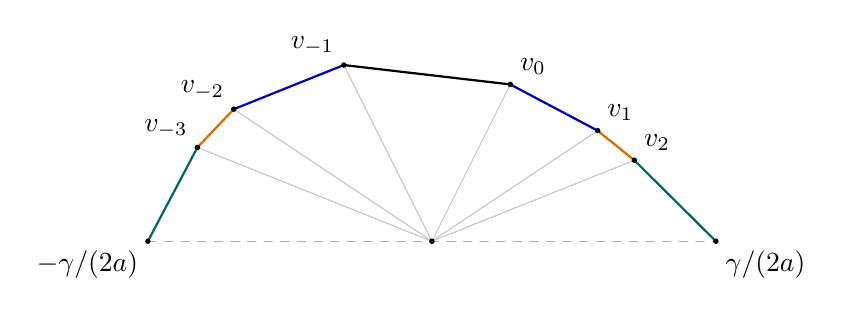
\begin{tikzpicture}[x=5cm,y=5cm,line cap=round]
% Coordinates computed in Python from the fan length formula.
% In the basis $(\gamma,\gamma'-\gamma/2)$,
% the vertex $v_n$ has coordinates $((n+1/2)/L_n,1/L_n)$,
% where $L_n$ is the length of $\gamma'+n\gamma$.
\coordinate (O)   at (0,0);
\coordinate (S-)  at (-0.721348,0);
\coordinate (V-3) at (-0.595598,0.238239);
\coordinate (V-2) at (-0.503171,0.335447);
\coordinate (V-1) at (-0.223772,0.447544);
\coordinate (V0)  at ( 0.199150,0.398300);
\coordinate (V1)  at ( 0.421226,0.280817);
\coordinate (V2)  at ( 0.514163,0.205665);
\coordinate (S+)  at ( 0.721348,0);

\draw[gray!65,dashed] (S-)--(S+);
\foreach \p in {V-3,V-2,V-1,V0,V1,V2}
  \draw[gray!45,thin] (O)--(\p);

% The middle edge, followed by the three pairs from the middle outward.
\draw[thick]                 (V-1)--(V0);
\draw[blue!70!black,thick]    (V-2)--(V-1) (V0)--(V1);
\draw[orange!85!black,thick]  (V-3)--(V-2) (V1)--(V2);
\draw[teal!80!black,thick]    (S-)--(V-3)  (V2)--(S+);

\foreach \p in {O,S-,V-3,V-2,V-1,V0,V1,V2,S+}
  \fill (\p) circle[radius=1pt];

\node[below left] at (S-) {$-\gamma/(2a)$};
\node[below right] at (S+) {$\gamma/(2a)$};
\foreach \n in {-3,-2,-1}
  \node[above left] at (V\n) {$v_{\n}$};
\foreach \n in {0,1,2}
  \node[above right] at (V\n) {$v_{\n}$};
\end{tikzpicture}
\caption{One half of the fan polygon for $M=2$, $a=\log 2$, and
$\theta=a/4$.}
\label{fig:fan-edge-pairing}
\end{figure}

\begin{theorem}[Short-systole estimate]
\label{thm:pure-cusp}
If $\sys(X)\leq7/5$, then $\A(X)>893/1000$.
\end{theorem}

\begin{proof}
Use the fan polygon with $M=2$ (Figure~\ref{fig:fan-edge-pairing}).
Set $\tau=\theta/a$ and list
the lengths in order as $\lambda=(2a,L_{-3},\ldots,L_2)$,
indexed from $0$ to $6$. Adjacent classes have determinant of
absolute value one, so the triangle at an edge and its opposite
have total area $1/(\lambda_i\lambda_{i+1})$. Thus
$$
\A(X)\geq P(a,\tau):=\sum_{i=0}^{6}\frac{1}{\lambda_i\lambda_{i+1}},
$$
with indices taken modulo $7$. Since changing the sign of $\tau$
reverses the fan, we may assume $0\leq\tau\leq1/2$.

Both $L_{-3}$ and $L_2$ are at most $l_a(3a)$, so the two terms
involving $2a$ give $P(a,\tau)\geq1/(a l_a(3a))$. If $a\leq9/40$,
then $\coth a>1/a\geq40/9>\cosh 1$, so $l_a(0)>2$.
Differentiating \eqref{eq:fan-length-function} gives
$\partial_a l_a(t)\geq-2/\sinh a\geq-2/a$. Since $l_a$ increases
with $t\geq0$, it follows that
$(a l_a(3a))'\geq l_a(3a)-2>0$.
Appendix~\ref{app:fan-interval-checks} gives $l_{9/40}(27/40)<49/10$,
so $P(a,\tau)>400/441$ on this range.

For each positive vector $r=(r_0,\ldots,r_6)$ and vector $w$ of
the same size, put
\begin{equation}
\label{eq:short-fan-tangent}
\Phi_r(w)=\sum_{i=0}^{6}
\frac{3-w_i/r_i-w_{i+1}/r_{i+1}}{r_i r_{i+1}}.
\end{equation}
The tangent inequality for the convex function $(x,y)\mapsto1/(xy)$
gives $P(a,\tau)\geq\Phi_r(\lambda)$.

Each component of $\lambda$ is convex in $a$ for fixed $\tau$ and in
$\tau$ for fixed $a$. The second assertion follows from
\eqref{eq:fan-curvature-function}. For the first, set
$b=\log\coth(a/2)$, so $\cosh b=\coth a$. The function
$\operatorname{arccosh}(\cosh b\cosh t)$ is the distance between
points parametrized by signed distance along two perpendicular
geodesics. Convexity of distance along geodesics in a
$\operatorname{CAT}(0)$ space gives convexity in $(b,t)$
\cite[Proposition~II.2.2, page~176]{BridsonHaefliger}.
The formula also shows that the distance increases with $b>0$.
Since $b''(a)=\cosh a/\sinh^2a>0$ and
$t=(n+1/2+\tau)a$ is affine in $a$, each $L_n$ is convex in $a$.

The affine function $\Phi_r$ decreases in each component.
Consequently $\Phi_r(\lambda)$ is concave in each of $a,\tau$
separately. Applying concavity first in $a$ and then in $\tau$ bounds
the function below by its smallest corner value on each rectangle.
Appendix~\ref{app:fan-interval-checks} covers
$[9/40,7/10]\times[0,1/2]$ by six rectangles and gives a vector $r$
for each one such that its four corner values exceed $893/1000$.
\end{proof}

\section{Proofs of the main theorems}
\label{sec:completion}

\begin{proposition}[Explicit regional estimate]
\label{prop:regional-area}
Every nonmodular torus $X$ satisfies
$$
\A(X)-\A(\Xmod)>
\begin{cases}
p_2/80,&\text{if }s_X\geq7/5,\\
1/1000,&\text{if }s_X<7/5.
\end{cases}
$$
\end{proposition}

\begin{proof}
For $s_X\geq7/5$, \eqref{eq:large-systole-comparison} gives the bound
$p_2/80$.
For $s_X<7/5$, Theorem~\ref{thm:pure-cusp} and
Proposition~\ref{prop:modular-upper-new} give
$$
\A(X)-\A(\Xmod)>\frac{893}{1000}-\frac{223}{250}=\frac1{1000}.
$$
\end{proof}

\begin{proof}[Proof of Theorem~\ref{thm:global-area}]
Since $p_2>0$ for every nonmodular torus,
Proposition~\ref{prop:regional-area} gives $\A(X)>\A(\Xmod)$.
The strict inequality between the leading coefficients in
\eqref{eq:Counting} gives $N_{\Xmod}(L)<N_X(L)$ for all sufficiently
large $L$.
\end{proof}

\begin{proof}[Proof of Theorem~\ref{thm:quantitative-area}]
Appendix~\ref{sec:cusp-growth} proves \eqref{eq:Expansion}.
For the global bounds, divide $\A(X)-\A(\Xmod)$
by $p_2e^{\sqrt{3p_2/2}}/(1+p_2)^{3/2}$ on the nonmodular tori.
As $p_2\to0$, the denominator is asymptotic to $p_2$, so the quotient
tends to $\kappa>0$ by Corollary~\ref{cor:modular-minimum}.

As $s_X\to0$, the discriminant inequality $\mathscr D(x,y)\geq0$,
Proposition~\ref{prop:markoff-reduction}, and reducedness give
$$
\frac{2}{\sqrt{x^2-4}}\leq\frac yx\leq\frac1{\sqrt{x-2}},
\qquad 1\leq\frac zy\leq\frac x2.
$$
Substituting $x=2\cosh(s_X/2)$ yields
$y/x=(2/s_X)(1+O(s_X^2))$ and $z/y=1+O(s_X^2)$.
Since $\log(z/x)=\log(y/x)+\log(z/y)$ and both summands are nonnegative,
\eqref{eq:p_2} gives
$$
\log(y/x)\leq\sqrt{3p_2/2}\leq\log(z/x),
$$
so $\sqrt{3p_2/2}=\log(2/s_X)+O(s_X^2)$.
Thus the denominator is asymptotic to
$\sqrt{6}/(s_X\log(2/s_X))$, and \eqref{eq:Expansion} gives
the limit $1/\sqrt{6}$ for the quotient.

After excluding a neighborhood of the modular point and all sufficiently
small systoles, the reduced triples form a compact set by the trace
bounds above and $x\leq3$. The quotient is continuous and positive there
by Theorem~\ref{thm:global-area}. Its two positive limits therefore give
the required bounds on all nonmodular tori. At the modular torus both
sides of each inequality are zero.
\end{proof}

\appendix
\section*{Appendix}
\addcontentsline{toc}{section}{Appendix}
% Number appendix parts independently of the main sections.
\renewcommand{\thesubsection}{A\arabic{subsection}}
\renewcommand{\theHsubsection}{appendix.\arabic{subsection}}
\renewcommand{\theHsubsubsection}{\theHsubsection.\arabic{subsubsection}}
\numberwithin{theorem}{subsection}
\renewcommand{\theHtheorem}{\theHsubsection.\arabic{theorem}}
\subsection{Elementary bounds for series remainders}
\label{app:series-estimates}

For a nonnegative integer $N$ and $0\leq t<N+2$,
\begin{equation}
\label{eq:exp-remainder}
0\leq e^t-\sum_{j=0}^{N}\frac{t^j}{j!}
\leq\frac{t^{N+1}}{(N+1)!}\frac1{1-t/(N+2)}.
\end{equation}
Indeed, after the first omitted term, the ratio of successive terms
is at most $t/(N+2)$, so their sum is bounded by a geometric series.

The same argument applied to the even terms gives, for real $t$ with
$t^2<(2N+3)(2N+4)$,
\begin{equation}
\label{eq:cosh-remainder}
0\leq\cosh t-\sum_{j=0}^{N}\frac{t^{2j}}{(2j)!}
\leq\frac{t^{2N+2}}{(2N+2)!}
\frac1{1-t^2/((2N+3)(2N+4))}.
\end{equation}
For example, $N=8$ gives $\cosh(118/125)<37/25$,
so $2\arccosh(3/2)>236/125$.

For the fan lengths at the interval endpoints, put
$$
\begin{aligned}
C(x)&=\sum_{j=0}^{12}\frac{x^{2j}}{(2j)!},&
S(x)&=\sum_{j=0}^{12}\frac{x^{2j+1}}{(2j+1)!},\\
C^+(x)&=C(x)+\frac{2x^{26}}{26!},&
S^+(x)&=S(x)+\frac{2x^{27}}{27!}.
\end{aligned}
$$
Then, for $0\leq x\leq5$,
\begin{equation}
\label{eq:fan-series-bounds}
C(x)\leq\cosh x\leq C^+(x),
S(x)\leq\sinh x\leq S^+(x).
\end{equation}
The ratios after the first omitted terms are at most
$25/(27\cdot28)$ and $25/(28\cdot29)$, respectively. Both are
less than $1/2$, so twice the first omitted term bounds each remainder.

For logarithms, let $v\geq1$ and put $u=(v-1)/(v+1)$. Then
$0\leq u<1$, and
\begin{equation}
\label{eq:log-remainder}
0\leq\log v-2\sum_{j=0}^{N}\frac{u^{2j+1}}{2j+1}
\leq\frac{2u^{2N+3}}{(2N+3)(1-u^2)}.
\end{equation}
Indeed, the logarithm series \cite[equation~(4.6.4)]{DLMF}
has terms $2u^{2j+1}/(2j+1)$. Replacing each omitted denominator
by $2N+3$ gives the geometric sum on the right. For any positive
argument, write it as $2^k v$ with $1\leq v<2$ and apply the bound
at $v$ and at $2$.

\subsection{Length bounds and Taylor coefficients of the polygon area}
\label{app:taylor-coefficients}

The polygon formula \eqref{eq:height-six-polygon-area} uses
$f(T)=1/L(T)$ with $L(T)=2\arccosh(T/2)$. We first bound these
lengths at the modular torus. The same bounds enter
Propositions~\ref{prop:modular-upper-new} and
\ref{prop:polygon-taylor-remainder}.

For each trace $T>2$ at the modular torus, put $D=10^{100}$ and define
$$
K_T=\max\{k\in\Z_{\geq0}:k^2\leq D^2(T^2-4)\}.
$$
Then
\begin{equation*}
K_T/D\leq\sqrt{T^2-4}\leq(K_T+1)/D.
\end{equation*}
Substitute these endpoints into $L(T)=2\log((T+\sqrt{T^2-4})/2)$
and apply \eqref{eq:log-remainder} with $N=99$ to bound $L(T)$.
For sums of intervals, add the lower and upper endpoints separately.
For products, take the smallest and largest of the four endpoint
products. For reciprocals, use $[a,b]^{-1}=[1/b,1/a]$ when
$0\notin[a,b]$. We may round the resulting endpoints outward to
$\lfloor Da\rfloor/D$ and $\lceil Db\rceil/D$.

\begin{lemma}[Explicit Taylor coefficient bounds]
\label{lem:explicit-low-coefficients}
\label{lem:higher-coefficients}
For the coefficients in \eqref{eq:invariant-homogeneous-form}, an entry $(a,b)$ means $a<1000c_{n,k}<b$.
A dash means that the coefficient does not occur.
\begingroup
\footnotesize
\setlength{\arraycolsep}{2pt}
\begin{equation}
\label{eq:taylor-coefficient-bounds}
\begin{array}{r|rrrr}
n&k=0&k=1&k=2&k=3\\
\hline
2&(115,116)&\text{--}&\text{--}&\text{--}\\
3&(-694,-692)&\text{--}&\text{--}&\text{--}\\
4&(-162,-161)&\text{--}&\text{--}&\text{--}\\
5&(812,815)&\text{--}&\text{--}&\text{--}\\
6&(-314,-312)&(6354,6367)&\text{--}&\text{--}\\
7&(270,277)&\text{--}&\text{--}&\text{--}\\
8&(1118,1128)&(-15077,-14964)&\text{--}&\text{--}\\
9&(2407,2408)&(-37499,-37498)&\text{--}&\text{--}\\
10&(-1373,-1372)&(14063,14064)&\text{--}&\text{--}\\
11&(-13233,-13232)&(135121,135122)&\text{--}&\text{--}\\
12&(985,986)&(-39829,-39828)&(286516,286517)&\text{--}\\
13&(22984,22985)&(-201453,-201452)&\text{--}&\text{--}\\
14&(-1948,-1947)&(185062,185063)&(-1374518,-1374517)&\text{--}\\
15&(-20400,-20399)&(405076,405077)&(-1909443,-1909442)&\text{--}\\
16&(6289,6290)&(-450043,-450042)&(3030012,3030013)&\text{--}\\
17&(31287,31288)&(-1786116,-1786115)&(11542319,11542320)&\text{--}\\
18&(-12548,-12547)&(721576,721577)&(-6517347,-6517346)&(14598450,14598451)\\
19&(-111754,-111753)&(5301317,5301318)&(-32106332,-32106331)&\text{--}\\
\end{array}
\end{equation}
\endgroup
\end{lemma}

\begin{proof}
Along each of the four directions $(a,b,c)=(1,-s,s-1)$ in
Lemma~\ref{lem:four-directions}, the parametrization
\eqref{eq:shape-trace-parametrization} gives
$$
x(t)=e^{3at}+2\cosh((b-c)t),
$$
with $y(t),z(t)$ obtained by cyclic permutation of $a,b,c$.
Their Taylor coefficients are rational. Keeping terms through degree
nineteen, compute the fan traces for each of the six permutations by
\eqref{eq:sector-trace-recursion} and use $T_*=T_1T_2-x$ for the
additional insertion.

For a trace series $x(t)=\sum_{j\geq0}x_jt^j$, let
$s_j,v_j,l_j,f_j$ be the Taylor coefficients of
$\sqrt{x(t)^2-4}$, its reciprocal, $L(x(t))$, and
$1/L(x(t))$, respectively. Their constant terms are
$$
s_0=\sqrt{x_0^2-4},
v_0=\frac1{s_0},
l_0=L(x_0),
f_0=\frac1{l_0}.
$$
Squaring the square-root series and multiplying reciprocal
pairs gives, for $1\leq j\leq19$,
\begin{equation*}
\begin{aligned}
s_j&=
\frac{\displaystyle\sum_{i=0}^jx_ix_{j-i}
-\displaystyle\sum_{i=1}^{j-1}s_is_{j-i}}{2s_0},\\
v_j&=-\frac1{s_0}\sum_{i=1}^js_iv_{j-i}.
\end{aligned}
\end{equation*}
Similarly, the chain rule
$(L(x(t)))'=2x'(t)/\sqrt{x(t)^2-4}$ and the reciprocal
identity give
\begin{equation*}
\begin{aligned}
l_j&=\frac2j\sum_{i=1}^ji x_iv_{j-i},\\
f_j&=-\frac1{l_0}\sum_{i=1}^jl_if_{j-i}.
\end{aligned}
\end{equation*}

Summing the products in \eqref{eq:height-six-polygon-area}
gives $H_n(1,-s,s-1)$ for $2\leq n\leq19$.
Substituting these values in \eqref{eq:one-variable-coefficient-polynomial}
and solving for $c_{n,k}$ gives intervals strictly inside the bounds in
\eqref{eq:taylor-coefficient-bounds}.
\end{proof}

\subsection{Verification of the numerical bounds}
\label{app:numerical-checks}

\subsubsection{The complex length bounds}
\label{app:complex-length-checks}

For $1\leq h\leq6$, the upper bound for $2\cosh(l_h/2)$ from
\eqref{eq:cosh-remainder} with $N=8$ is less than the corresponding
lower bound for $|x_w|$ in \eqref{eq:complex-height-trace-bounds}.
This verifies \eqref{eq:complex-length-lower-bounds}.

\subsubsection{Corner checks for the fan polygon}
\label{app:fan-interval-checks}

Use the polynomials in \eqref{eq:fan-series-bounds}. The inequality
$$
S(9/40)C(49/20)>C^+(9/40)C^+(27/40)
$$
gives $l_{9/40}(27/40)<49/10$. For the remaining checks take
consecutive intervals with endpoints in the ordered lists
$$
(a_0,a_1,a_2,a_3)=(9/40,11/25,3/5,7/10)
\text{ and }(\tau_0,\tau_1,\tau_2)=(0,1/4,1/2).
$$
At a corner $(a,\tau)$, form the vector
$u(a,\tau)=(2a,U_{-3},\ldots,U_2)$, where $U_n$ is the least positive
multiple of $10^{-4}$ at most $10$ for which
$$
S(a)C(U_n/2)>C^+(a)C^+(|(n+1/2+\tau)a|).
$$
Such a multiple exists since
$S(9/40)C(5)>C^+(7/10)C^+(21/10)$. By
\eqref{eq:fan-series-bounds} and \eqref{eq:fan-length-function},
$U_n>L_n$.

On $[a_i,a_{i+1}]\times[\tau_j,\tau_{j+1}]$, take $r$ to be
the average of $u(a_{i+1},\tau_j)$ and $u(a_{i+1},\tau_{j+1})$.
Since $\Phi_r$ decreases in each component, the corner values
$\Phi_r(u(a,\tau))$ bound $\Phi_r(\lambda)$ from below there.
Substitution into \eqref{eq:short-fan-tangent} gives the following
strict lower bounds for $1000\Phi_r(u(a,\tau))$ at all four corners.
$$
\begin{array}{c|rr}
[a_i,a_{i+1}] & [0,1/4] & [1/4,1/2] \\ \hline
{[9/40,11/25]} & 899 & 898 \\
{[11/25,3/5]} & 899 & 898 \\
{[3/5,7/10]} & 894 & 894
\end{array}
$$
All comparisons involve only rational numbers.

\subsection{Proof of the cusp expansion}
\label{sec:cusp-growth}

Use the fan of Subsection~\ref{sec:global} and set $b=\log\coth a$.
All estimates below are uniform in the twist. Let $\A_{\mathrm{fan}}$
be the limit of the areas of the nested fan polygons. The contributions
of the edges incident to the systole vertices tend to zero because
$L_n\to\infty$ as $|n|\to\infty$.
Let $\widetilde l_a$ interpolate $l_a$ linearly at the points
$(n+1/2)a+\theta$. On an interval with endpoint values $L_n,L_{n+1}$,
the integral of $\widetilde l_a^{-2}$ is $a/(L_nL_{n+1})$. Thus
$$
\A_{\mathrm{fan}}=\sum_{n\in\Z}\frac1{L_nL_{n+1}}
=\frac1a\int_{\R}\frac{dt}{\widetilde l_a(t)^2}.
$$

For $t\geq0$, put $g(t)=\log(1+e^{-2t})$. By
\eqref{eq:fan-length-function} and
$\arccosh x=\log(2x)+O(x^{-2})$, we have
$l_a(t)=2(b+|t|+g(|t|))+O(a^2)$ uniformly in $t$.
The bound $0<l_a''\leq2\cosh a$ from
\eqref{eq:fan-curvature-function} gives $\widetilde l_a-l_a=O(a^2)$.
Since $\cosh(b+|t|)\leq\coth a\cosh t$ and $l_a$ is convex,
$\widetilde l_a(t)\geq l_a(t)\geq2(b+|t|)$.
In particular, $\A_{\mathrm{fan}}\leq1/(2ab)$.
The difference between the reciprocal squares of $\widetilde l_a(t)$
and $2(b+|t|+g(|t|))$ is $O(a^2(b+|t|)^{-3})$. Integrating gives
$$
\A_{\mathrm{fan}}
=\frac1{2a}\int_0^\infty\frac{dt}{(b+t+g(t))^2}+O(a/b^2).
$$

To estimate the area outside the fan triangles, consider successive
Farey insertions between two consecutive fan classes $u,v$.
If $x_{u-v}\leq\max(x_u,x_v)$, then \eqref{eq:vieta} gives
$x_{u+v}>\max(x_u,x_v)$ because $\min(x_u,x_v)>2$.
This condition holds at the first edge since $v-u=\gamma$ is a
systole. It persists at each new edge because the trace across it
is an old endpoint trace, smaller than the newly inserted trace.
Each insertion therefore takes the larger root of \eqref{eq:2trace}, and all lengths are at least
$l_a(0)\geq2b$. For sufficiently small $a$,
Proposition~\ref{prop:scalar-defect} bounds each length deficit by
$11e^{-2l_a(0)}=O(a^4)$, since $e^{-b}=\tanh a$.

For coprime positive integers $p,q$, induction on the insertions gives
$$
\|pu+qv\|_X\geq pL_u+qL_v-O((p+q-1)a^4).
$$
Since $L_u,L_v\geq2b$, the norm is at least
$(1-O(a^4/b))(pL_u+qL_v)$, and this bound extends to real $p,q\geq0$
by homogeneity and continuity.
The fan triangle in this sector is cut out by $pL_u+qL_v\leq1$.
A dilation by a factor $1+O(a^4/b)$ therefore encloses the part of
$\B_X$ in that sector. Summing the areas gives
$$
0\leq\A(X)-\A_{\mathrm{fan}}
=O(a^4/b)\A_{\mathrm{fan}}=O(a^3/b^2).
$$

Since $g(t)\leq e^{-2t}$, both $g(t)^2$ and $tg(t)$ are integrable.
Taylor expansion in $g(t)$ and
$|(b+t)^{-3}-b^{-3}|\leq3t/b^4$ give
$$
\int_0^\infty\frac{dt}{(b+t+g(t))^2}
=\frac1b-\frac{2}{b^3}\int_0^\infty g(t)dt+O(b^{-4}).
$$
Integrating the logarithm series gives
$\int_0^\infty g(t)dt=\frac12\sum_{j\geq1}(-1)^{j+1}/j^2=\pi^2/24$.
The interpolation error and the area outside the fan are $o(1/(ab^4))$.
Substituting $s_X=2a$ and $b=\log(1/a)+O(a^2)$ gives \eqref{eq:Expansion}.
Since $ab^4\to0$, subtracting the fixed area $\A(\Xmod)$ gives the
same expansion.

\small
\begin{thebibliography}{MR95b}

\bibitem[Akr03]{Akrout2003}
H. Akrout,
Singularit\'es topologiques des systoles g\'en\'eralis\'ees,
\emph{Topology} \textbf{42} (2003), no. 2, 291--308,
\url{https://doi.org/10.1016/S0040-9383(01)00024-6}.

\bibitem[AA26]{AougabAthreya}
T. Aougab and J. S. Athreya,
Currents with corners and counting weighted triangulations,
\emph{J. Lond. Math. Soc.} \textbf{114} (2026), e70675,
\url{https://doi.org/10.1112/jlms.70675}.

\bibitem[AHA20]{AranaHerreraAthreya}
F. Arana-Herrera and J. S. Athreya,
Square-integrability of the Mirzakhani function and statistics of simple
closed geodesics on hyperbolic surfaces,
\emph{Forum Math. Sigma} \textbf{8} (2020), e9, 33 pp.,
\url{https://doi.org/10.1017/fms.2019.49}.

\bibitem[BM17]{BabenkoMassart2017}
I. Babenko and D. Massart,
On systolic zeta functions,
\emph{European Journal of Mathematics} \textbf{3} (2017), 899--915,
\url{https://doi.org/10.1007/s40879-017-0181-1}.

\bibitem[BK03]{BangertKatz}
Victor Bangert and Mikhail Katz,
Stable systolic inequalities and cohomology products,
\emph{Communications on Pure and Applied Mathematics}
\textbf{56} (2003), no. 7, 979--997,
\url{https://doi.org/10.1002/cpa.10082}.

\bibitem[Bel23]{Bell}
N. Bell,
Counting arcs on hyperbolic surfaces,
\emph{Groups Geom. Dyn.} \textbf{17} (2023), no. 2, 459--478,
\url{https://doi.org/10.4171/GGD/705}.

\bibitem[Bon18]{Bonahon2018}
F. Bonahon,
\emph{The Mirzakhani function on the moduli space of a surface},
recorded lecture at the 2018 Fields Medal Symposium: Maryam Mirzakhani,
Fields Institute, Toronto, November 7, 2018,
reporting joint work with Sabrina Enriquez,
\url{https://www.fields.utoronto.ca/talks/Mirzakhani-function-moduli-space-surface}.

\bibitem[BW11]{BonahonWong2011}
F. Bonahon and H. Wong,
Quantum traces for representations of surface groups in
$\mathrm{SL}_2(\mathbb C)$,
\emph{Geometry \& Topology} \textbf{15} (2011), 1569--1615,
\url{https://doi.org/10.2140/gt.2011.15.1569}.

% \bibitem[BCD+23]{BorotEtAlUnitBall}
% G. Borot, S. Charbonnier, V. Delecroix, A. Giacchetto, and C. Wheeler,
% Around the combinatorial unit ball of measured foliations on bordered surfaces,
% \emph{Int. Math. Res. Not. IMRN} \textbf{2023} (2023), no. 17,
% 14464--14514,
% \url{https://doi.org/10.1093/imrn/rnac231}.

\bibitem[BMMR13]{BoroczkyMakaiMeyerReisner}
K. J. B\"or\"oczky, E. Makai, Jr., M. Meyer, and S. Reisner,
On the volume product of planar polar convex bodies---lower
estimates with stability,
Studia Scientiarum Mathematicarum Hungarica
\textbf{50} (2013), no.~2, 159--198,
\url{https://doi.org/10.1556/SScMath.50.2013.2.1235}.

\bibitem[Bow98]{Bowditch}
B. H. Bowditch,
Markoff triples and quasifuchsian groups,
\emph{Proc. Lond. Math. Soc.} (3) \textbf{77} (1998), no. 3, 697--736,
\url{https://doi.org/10.1112/S0024611598000604}.


\bibitem[BH99]{BridsonHaefliger}
M. R. Bridson and A. Haefliger,
\emph{Metric Spaces of Non-Positive Curvature},
Grundlehren der mathematischen Wissenschaften \textbf{319},
Springer, Berlin, 1999,
\url{https://doi.org/10.1007/978-3-662-12494-9}.

\bibitem[Cas59]{Cassels}
J. W. S. Cassels,
\emph{An Introduction to the Geometry of Numbers},
Grundlehren der mathematischen Wissenschaften, vol. 99,
Springer-Verlag, Berlin, 1959.

\bibitem[Che25]{Chen2025Morse}
C. Chen,
Morse theory on moduli of curves,
preprint, arXiv:2307.16119v4, 2025,
\url{https://arxiv.org/abs/2307.16119v4}.

\bibitem[DGZZ21]{DelecroixGoujardZografZorich}
V. Delecroix, \'E. Goujard, P. Zograf, and A. Zorich,
Masur--Veech volumes, frequencies of simple closed geodesics, and
intersection numbers of moduli spaces of curves,
\emph{Duke Math. J.} \textbf{170} (2021), no. 12, 2633--2718,
\url{https://doi.org/10.1215/00127094-2021-0054}.

\bibitem[DLMF]{DLMF}
National Institute of Standards and Technology,
\emph{Digital Library of Mathematical Functions},
\url{https://dlmf.nist.gov/}.

\bibitem[DLN26]{DLN}
N. M. Doan, X. Li, and V. Nguyen,
Stable-norm boundary geometry on once-punctured tori,
arXiv:2605.14574, version 3, 2026,
\url{https://arxiv.org/abs/2605.14574v3}.

\bibitem[ES16]{ErlandssonSouto}
V. Erlandsson and J. Souto,
Counting curves in hyperbolic surfaces,
\emph{Geom. Funct. Anal.} \textbf{26} (2016), no. 3, 729--777,
\url{https://doi.org/10.1007/s00039-016-0374-7}.

\bibitem[ES22]{ErlandssonSoutoBook}
V. Erlandsson and J. Souto,
\emph{Mirzakhani's Curve Counting and Geodesic Currents},
Progress in Mathematics \textbf{345}, Birkh\"auser, Cham, 2022,
\url{https://doi.org/10.1007/978-3-031-08705-9}.

\bibitem[Fed74]{Federer1974}
H. Federer,
Real flat chains, cochains and variational problems,
\emph{Indiana Univ. Math. J.} \textbf{24} (1974/75), 351--407.

\bibitem[FM12]{FarbMargalit}
B. Farb and D. Margalit,
\emph{A Primer on Mapping Class Groups},
Princeton Mathematical Series \textbf{49}, Princeton University Press,
Princeton, 2012.

\bibitem[FMZ23]{FradeliziMeyerZvavitch}
M. Fradelizi, M. Meyer, and A. Zvavitch,
Volume product,
in \emph{Harmonic Analysis and Convexity},
De Gruyter, 2023, 163--223,
\url{https://arxiv.org/abs/2301.06131}.


\bibitem[Gol09]{GoldmanTrace}
W. M. Goldman,
Trace coordinates on Fricke spaces of some simple hyperbolic surfaces,
in \emph{Handbook of Teichm\"uller Theory}, Vol. II,
IRMA Lect. Math. Theor. Phys. \textbf{13}, European Mathematical Society,
Z\"urich, 2009, 611--684,
\url{https://doi.org/10.4171/055-1/16}.

\bibitem[GN12]{GorodnikNevo}
A. Gorodnik and A. Nevo,
Counting lattice points,
\emph{J. Reine Angew. Math.} \textbf{663} (2012), 127--176,
\url{https://doi.org/10.1515/CRELLE.2011.096}.

\bibitem[Gro83]{Gromov1983}
M. Gromov,
Filling Riemannian manifolds,
\emph{J. Differential Geom.} \textbf{18} (1983), no. 1, 1--147,
\url{https://doi.org/10.4310/jdg/1214509283}.

\bibitem[HT14]{HuTan}
H. Hu and S. P. Tan,
\emph{New identities for small hyperbolic surfaces},
Bull. Lond. Math. Soc. \textbf{46} (2014), no.~5, 1021--1031.

\bibitem[IS26]{IrmerSaha2026}
I. Irmer and B. N. Saha,
The diameter function is a topological Morse function,
preprint, arXiv:2606.21291, 2026,
\url{https://arxiv.org/abs/2606.21291}.

\bibitem[Iva15]{Ivaki}
M. N. Ivaki,
Stability of the Blaschke--Santal\'o inequality in the plane,
Monatshefte f\"ur Mathematik
\textbf{177} (2015), no.~3, 451--459,
\url{https://doi.org/10.1007/s00605-014-0651-1}.

\bibitem[LMN26]{LoweMarquesNeves}
B. Lowe, F. C. Marques, and A. Neves,
Counting minimal Lagrangians via Mirzakhani functions,
arXiv:2605.04614, version 3, 2026,
\url{https://arxiv.org/abs/2605.04614v3}.

\bibitem[Mac95]{Macdonald}
I. G. Macdonald,
\emph{Symmetric Functions and Hall Polynomials}, second edition,
Oxford Mathematical Monographs, Clarendon Press, Oxford, 1995.

\bibitem[Mah38]{Mahler}
K. Mahler,
Ein Minimalproblem f\"ur convexe Polygone,
Mathematica (Zutphen) B \textbf{7} (1938), 118--127.

\bibitem[MP90]{MeyerPajor}
M. Meyer and A. Pajor,
On the Blaschke--Santal\'o inequality,
Archiv der Mathematik \textbf{55} (1990), 82--93,
\url{https://doi.org/10.1007/BF01199119}.

\bibitem[Mir08a]{MirzakhaniGrowth}
M. Mirzakhani,
Growth of the number of simple closed geodesics on hyperbolic surfaces,
\emph{Ann. of Math.} (2) \textbf{168} (2008), no. 1, 97--125,
\url{https://doi.org/10.4007/annals.2008.168.97}.

\bibitem[Mir08b]{MirzakhaniEarthquake}
M. Mirzakhani,
Ergodic theory of the earthquake flow,
\emph{Int. Math. Res. Not. IMRN} \textbf{2008} (2008),
Art. ID rnm116, 39 pp.,
\url{https://doi.org/10.1093/imrn/rnm116}.


\bibitem[Mir16]{MirzakhaniOrbits}
M. Mirzakhani,
Counting mapping class group orbits on hyperbolic surfaces,
arXiv:1601.03342, 2016,
\url{https://arxiv.org/abs/1601.03342}.

\bibitem[MR95a]{McShaneRivinNorm}
G. McShane and I. Rivin,
A norm on homology of surfaces and counting simple geodesics,
\emph{Internat. Math. Res. Notices} \textbf{1995} (1995), no. 2, 61--69,
\url{https://doi.org/10.1155/S1073792895000055}.

\bibitem[MR95b]{McShaneRivinTori}
G. McShane and I. Rivin,
Simple curves on hyperbolic tori,
\emph{C. R. Acad. Sci. Paris S\'er. I Math.} \textbf{320} (1995), no. 12,
1523--1528; electronic text corresponding to the published article:
arXiv:math/0005220.

\bibitem[Mor59]{Morse1959}
M. Morse,
Topologically non-degenerate functions on a compact $n$-manifold $M$,
\emph{J. Anal. Math.} \textbf{7} (1959), 189--208,
\url{https://doi.org/10.1007/BF02787685}.

\bibitem[O'S26]{OSullivan2026}
C. O'Sullivan,
Patterns in the Markov numbers and their generalizations,
arXiv:2609.14149, 2026,
\url{https://arxiv.org/abs/2609.14149}.

\bibitem[OAI26]{OpenAIMahler}
OpenAI,
\emph{The symmetric Mahler conjecture and its equality cases},
preprint released in the OpenAI math collection, 2026,
\url{https://github.com/openai/math/blob/main/preprints/The-symmetric-Mahler-conjecture-and-its-equality-cases-September-22-2026/paper.pdf}.

\bibitem[Pal79]{Palais1979}
R. S. Palais,
The principle of symmetric criticality,
\emph{Communications in Mathematical Physics}
\textbf{69} (1979), no. 1, 19--30.

\bibitem[PP98]{ParkerParkkonen1998}
J. R. Parker and J. Parkkonen,
Coordinates for quasi-Fuchsian punctured torus space,
\emph{Geom. Topol. Monogr.} \textbf{1} (1998), 451--478,
\url{https://arxiv.org/abs/math/9810199}.

\bibitem[Par99]{Parkkonen1999}
J. Parkkonen,
The outside of the Teichm\"uller space of punctured tori in
Maskit's embedding,
\emph{Annales Academi\ae{} Scientiarum Fennic\ae{} Mathematica}
\textbf{24} (1999), 305--342,
\url{https://www.acadsci.fi/mathematica/Vol24/parkkone.pdf}.

\bibitem[Par14]{ParlierSurvey}
H. Parlier,
Simple closed geodesics and the study of Teichm\"uller spaces,
in \emph{Handbook of Teichm\"uller Theory}, Vol. IV,
IRMA Lect. Math. Theor. Phys. \textbf{19}, European Mathematical Society,
Z\"urich, 2014, 113--134,
\url{https://doi.org/10.4171/117-1/3}.

\bibitem[RS19]{RafiSouto}
K. Rafi and J. Souto,
Geodesic currents and counting problems,
\emph{Geom. Funct. Anal.} \textbf{29} (2019), 871--889,
\url{https://doi.org/10.1007/s00039-019-00502-7}.

\bibitem[Rei86]{Reisner}
S. Reisner,
Zonoids with minimal volume-product,
Mathematische Zeitschrift \textbf{192} (1986), 339--346,
\url{https://doi.org/10.1007/BF01164009}.

\bibitem[Ris26]{Risager2026}
M. S. Risager,
Counting Markov triples and simple geodesics,
arXiv:2610.36069, version 1, 2026,
\url{https://arxiv.org/abs/2610.36069v1}.

\bibitem[Rud76]{Rudin}
W. Rudin,
\emph{Principles of Mathematical Analysis}, third edition,
McGraw--Hill, New York, 1976.

\bibitem[Sas25]{Sasaki}
D. Sasaki,
Counting subgroups via Mirzakhani's curve counting,
arXiv:2409.08109, version 3, 2025,
\url{https://arxiv.org/abs/2409.08109v3}.

\bibitem[Sch93]{Schmutz}
P. Schmutz,
\emph{Riemann surfaces with shortest geodesic of maximal length},
Geometric and Functional Analysis \textbf{3} (1993), 564--631.

\bibitem[Sch99]{SchmutzSchaller1999}
P. Schmutz Schaller,
Systoles and topological Morse functions for Riemann surfaces,
\emph{J. Differential Geom.} \textbf{52} (1999), no. 3, 407--452.

\bibitem[Sch14]{Schneider}
R. Schneider,
\emph{Convex Bodies: The Brunn--Minkowski Theory}, second expanded edition,
Encyclopedia of Mathematics and its Applications \textbf{151},
Cambridge University Press, Cambridge, 2014.

\bibitem[SS03a]{SteinShakarchiFourier}
E. M. Stein and R. Shakarchi,
\emph{Fourier Analysis: An Introduction},
Princeton Lectures in Analysis, vol. I,
Princeton University Press, Princeton, 2003.

\bibitem[SS03b]{SteinShakarchi}
E. M. Stein and R. Shakarchi,
\emph{Complex Analysis},
Princeton Lectures in Analysis, vol. II,
Princeton University Press, Princeton, 2003.

\bibitem[TZ26]{TanZhang26}
H. Tan and Y. Zhang,
\emph{The modular torus maximizes the Mahler product of the stable norm ball},
preprint, 2026,
\url{https://doi.org/10.5281/zenodo.23603543}.

\bibitem[Thu98]{ThurstonMinimalStretch}
W. P. Thurston,
Minimal stretch maps between hyperbolic surfaces,
preprint, 1986, posted as arXiv:math/9801039 in 1998,
\url{https://arxiv.org/abs/math/9801039}.

\bibitem[Tri24]{Trin}
M. Trin,
Counting arcs of the same type,
\emph{Int. Math. Res. Not. IMRN} \textbf{2024} (2024),
no. 16, 11749--11765,
\url{https://doi.org/10.1093/imrn/rnae143}.

\bibitem[Wol87]{Wolpert1987}
S. A. Wolpert,
Geodesic length functions and the Nielsen problem,
\emph{J. Differential Geom.} \textbf{25} (1987), no. 2, 275--296,
\url{https://doi.org/10.4310/jdg/1214440853}.

\bibitem[Zag82]{Zagier1982}
D. Zagier,
On the number of Markoff numbers below a given bound,
\emph{Math. Comp.} \textbf{39} (1982), no. 160, 709--723,
\url{https://doi.org/10.1090/S0025-5718-1982-0669663-7}.

\end{thebibliography}

\bigskip
\noindent
\begin{minipage}{\textwidth}
\small
\textsc{Phuc Thinh Dang}\par
Vietnam National University, Ho Chi Minh City, Vietnam\par
\textit{Email address:} 
\href{mailto:dpthinhmaths@gmail.com}{\nolinkurl{dpthinhmaths@gmail.com}}
\end{minipage}

\medskip
\noindent
\begin{minipage}{\textwidth}
\small
\textsc{Trong Toan Dao}\par
National University of Singapore, Singapore \par
\textit{Email address:}
\href{mailto:daotrongtoan.dtt4@gmail.com}{\nolinkurl{daotrongtoan.dtt4@gmail.com}} and \href{mailto:daotrongtoan@u.nus.edu}{\nolinkurl{daotrongtoan@u.nus.edu}}
\end{minipage}

\medskip
\noindent
\begin{minipage}{\textwidth}
\small
\textsc{Nhat Minh Doan}\par
Institute of Mathematics, Vietnam Academy of Science and Technology,
Hanoi, Vietnam\par
\textit{Email address:}
\href{mailto:dnminh@math.ac.vn}{\nolinkurl{dnminh@math.ac.vn}}\par
\textit{URL:}
\href{https://minhmath.github.io}{\nolinkurl{https://minhmath.github.io}}
\end{minipage}
\end{document}
